\documentclass{report}
\usepackage[utf8]{inputenc}
\usepackage{graphicx}
\usepackage{amsmath,amssymb}
\usepackage{hyperref}
\usepackage{geometry}
\usepackage{titlesec}
\usepackage{listings}
\usepackage{pythonhighlight}
\usepackage{fancyhdr}
\usepackage{setspace}
\usepackage{csquotes}
\usepackage[T1]{fontenc}
\usepackage[style=authoryear-ibid,backend=biber]{biblatex}
\addbibresource{UoR_Masters_Project.biblatex}

% Page settings
\geometry{margin=1in}
\setlength{\parskip}{0.8em}
\setlength{\parindent}{0pt}
\doublespacing% Header and Footer
\pagestyle{fancy}
\fancyhf{}
\rhead{\thepage}
\lhead{ML-Powered Agile PM App}

% Title
\title{\textbf{An LLM-Powered Application for Agile Project Management}}
\author{Nithin Gandhi Simanand \\ Supervisor: Pat Parslow \\ MSc Data Science and Advanced Computing}
\date{\today}

\begin{document}

\maketitle

\tableofcontents

\newpage

% 1. Introduction
\chapter{Introduction}  % ~800 words
\section{Problem Statement and Motivation}

Enterprise-scale organisations routinely operate across a complex matrix of interdependent projects, movement across teams, and extensive resource portfolios.
To maintain operational coherence and deliver value efficiently these firms typically rely on structured project management frameworks such as PRINCE2, PMBOK, or Agile-based hybrids. 
While such methodologies have demonstrated clear benefits in improving project visibility, governance, and stakeholder alignment, they remain susceptible to inherent inefficiencies. 
These stem largely from the rigidities of hierarchical communication, bureaucratic inertia, and the sheer scale of coordination required in large corporate environments \parencite{pricaEnhancingProjectEfficiency2025}.

Despite adherence to best practices, many firms continue to experience avoidable project delays, resource misallocation, and suboptimal decision-making cycles \parencite{mankinsTurningGreatStrategy2005}. 
A significant portion of these inefficiencies can be traced to human limitations in managing high-dimensional data, repetitive administrative tasks, and the cognitive overload associated with large-scale project orchestration. 
This presents a critical bottleneck: even with mature frameworks in place, enterprise project management often lacks the real-time adaptability and computational agility required to fully optimise performance at scale.

The emergence of Large Language Models (LLMs) and Machine Learning (ML) systems offers a transformative opportunity to address these structural inefficiencies. 
These technologies excel at pattern recognition, predictive analysis, and automating low-level cognitive functions, all attributes that align closely with the pain points of modern project management. 
By offloading repetitive, computation-heavy, and data-intensive components of project workflows to intelligent systems, organisations can enable human stakeholders to concentrate on strategic, creative, and high-context tasks where human judgment is irreplaceable.

However, due to the ever-growing importance of data protection, firms are increasingly hesitant to integrate cloud-based AI providers into their workflows. 
Concerns surrounding the ambiguity of how data is processed, where it is transmitted, and which datasets were used to train these models have created a significant barrier to adoption. 
While some organisations attempt to mitigate this risk by deploying locally hosted LLMs, these models typically function as open-ended chatbots. 
Consequently, the quality and relevance of their outputs are highly dependent on the user's ability to craft precise, context-aware prompts. 
Given the diversity in LLM interfaces, capabilities, and task specialisation, employees without training in prompt engineering or a deep understanding of model behavior often struggle to extract meaningful value, effectively neutralising the potential gains these tools could offer.

This research is motivated by the need to bridge the gap between the theoretical capabilities of intelligent automation systems and their practical usability in real-world enterprise settings. 
The core problem lies not only in technical implementation, but also in aligning these systems with organisational workflows, ensuring security and compliance, and designing interfaces and processes that make advanced tools accessible to non-expert users.
The goal is to explore how LLM- and ML-driven solutions can be securely, effectively, and intuitively integrated into large-scale project environments enabling genuine improvements in efficiency, responsiveness, and decision quality as well as ensuring projects are deliveres on time without compromising data integrity or overwhelming the workforce.

\section{Project Objectives}

There are four main objectives for this project:
\subsection{Develop a Multi-Dimensional Sprint Planner}
The first goal is to design an intelligent sprint planning system that automates the prioritisation and scheduling of project tasks. 
This planner considers multiple dynamic inputs, including team member availability, skill sets, task dependencies, organisational constraints, and regulatory and compliance related deadlines. 
The system is built to continuously ingest real-time updates, allowing it to refine project roadmaps dynamically as requirements shift. 
By embedding adaptive logic into the planner, the tool ensures that large-scale delivery remains aligned with strategic goals and operational timelines.

\subsection{Implement an Eisenhower Matrix-Based To-Do List Generator}
To enhance daily execution at the individual level, the system generates personalised task lists using the Eisenhower Matrix framework. 
This model categorises tasks based on urgency and importance, helping users focus on high-impact work while deferring or delegating less critical activities. 
These lists are continuously updated based on project context and user input and allowing users to identify high leverage activities without manual task sorting

\subsection{Integrate a Version Control System with LLM-Generated Commit Summaries}
The third objective is to ensure knowledge continuity and reduce the cognitive cost of context switching by embedding a version control system (VCS) into the platform. 
The VCS tracks project artefacts, decisions, and revisions, while an LLM generates automatic commit summaries that document key changes in clear, concise language. 
These summaries can be aggregated into progress reports, streamlining communication with internal stakeholders and external clients. 
Additionally, the system surfaces relevant historical context during task transitions, reducing ramp-up time and minimising productivity losses across team handovers or project shifts.
\subsection{Ensure Secure, Containerised Local Deployment}
Finally, the project emphasises data security and deployment flexibility by containerising the entire application for on-premise use. 
This architecture ensures that all data processing occurs within the organisation's infrastructure, mitigating the risks associated with cloud-based AI platforms. 
The modular software design also supports plug-and-play integration of different LLMs for specialised tasks, allowing components to be updated independently without disrupting the user experience. 
By abstracting LLM interactions behind clearly defined workflows, the system eliminates the need for prompt engineering, making advanced AI capabilities accessible to non-technical users.

Testing for this project will focus on validating both functional performance and usability across the four core components. 
For the multi-dimensional sprint planner, tests will assess the accuracy and adaptability of task prioritisation and scheduling in response to simulated changes in team availability, task dependencies, and deadlines. 
The Eisenhower Matrix task generator will be evaluated on its ability to categorise tasks correctly based on urgency and importance, as well as its impact on user focus and task completion rates.
The version control system and commit summarisation feature will be tested for robustness in tracking file changes, accuracy of LLM-generated summaries, and their usefulness in aiding project recall and progress reporting. 
The specific details of the testing methodology will be outlined in the Methodology chapter with greater detail of the test cases available in Appendix \ref{app:Scripts}.

% 2. Background & Literature Review
\chapter{Background and Literature Review}  % ~2000 words
\section{Project Management}

As this software project aims to assist enterprise-level organisations with project management, it is vital for it to interface with companies' existing project management frameworks. 
This means ensuring that the workflow of the software does not in itself become a barrier to adoption, necessitating software-specific training and introducing new inefficiencies as a result.

In order to ascertain which framework would be the best to start working with, `Analysis and Comparison of Project Management Standards and Guides' was reviewed \parencite{xueAnalysisComparisonProject}.
Xue et.\ al.\ sets out to analyse and compare three prominent PM references (PMBoK, ISO 21500, and ISO/IEC 29110) to assist project managers in making an informed choice, tailored to the scale of their project and its needs.

The motivation behind the study is grounded in the evolution of project management practices and the increasing need for clear guidance, especially in a landscape where projects vary vastly in size, complexity, and organisational structure. 
The paper begins by providing a historical context, illustrating that project management (PM) has been practised for millennia, and has continuously evolved with tools like Gantt charts, The Critical Path Method (CPM), Work Breakdown Structure (WBS), and Earned Value Management (EVM) becoming integral to contemporary PM. 
However, the variety of standards and guides, each designed with different target audiences, creates confusion for project managers, especially those unfamiliar with the subtle differences or lacking the time to conduct deep comparative analysis.

The analysis and comparison conducted directly responds to its problem statement by reducing the complexity around PM standard selection, thereby facilitating better adoption of PM practices tailored to project and organisational size. 
Furthermore, the paper's discussion about the trend of large companies outsourcing to smaller suppliers underscores the growing importance of matching standards to organisational scale, especially as supply chains become more fragmented.

To gain a greater understanding, more research was conducted to identify the different project management methodologies used in industry. 
Reading `Analysis of the Available Project Management Methodologies' \parencite{jovanovicAnalysisAvailableProject2018} once again highlighted that the effective implementation of project management methodologies remains a critical concern for organisations. 
Jovanovic et.\ al.\ address a well-documented challenge in project management literature: the inadequacy of one-size-fits-all methodologies to accommodate the heterogeneous nature of projects across different sectors and scales.

The paper's problem statement identifies a key gap: while numerous internationally recognised methodologies offer structured frameworks and processes, they often fail to consider the unique attributes of particular project types. 
This limitation is especially salient given the wide variance in project complexity, scope, and sector-specific needs. 
Agile methodologies emerge from the analysis as particularly well-suited to smaller, less complex projects, especially within the IT sector. 
Their iterative and flexible nature accommodates rapid change and uncertainty, addressing deficiencies in traditional methodologies, when applied to dynamic or fast-paced project environments. 
However, Xue et.\ al.\ find Agile's applicability outside IT and similarly scoped projects remains limited.

The study's synthesis underscores a critical implication: the suitability of any project management methodology is contingent on the interplay between project type, organisational culture, and management philosophy.
This reinforces the necessity of moving beyond generalised processes towards methodologies that reflect the specific demands and contexts of project groups.  

The research alludes to future / further development of a modular system that can interface with a range of different project management processes, ensuring that the correct framework is used for the nature of each project and the team members involved whilst also ensuring that data flows smoothly between different projects following different management protocols.

A stand out point here is the claim made by Xue et.\ al.\ that the efficacy of Agile is limited. 
Serrador and Pinto explore the tangible impact of Agile methodologies on project success, offering empirical evidence to support the growing adoption of Agile practices in contemporary project management \parencite{serradorDoesAgileWork2015}. 
The core aim of the study is to assess whether the degree of Agile usage in a project is positively correlated with various dimensions of project success, namely overall success, efficiency (time and budget), and stakeholder satisfaction. 
This objective is positioned within a broader critique of the historically high failure rates of projects despite adherence to traditional methodologies, such as waterfall.

The paper is underpinned by data from 1,386 projects across various industries, providing a substantial empirical base. 
The methodology quantifies the extent of Agile implementation on a scale from 0\% to 100\% and measures its correlation with perceived project outcomes. 
The results reveal a statistically significant, though modest, positive relationship between Agile usage and project success, especially in terms of stakeholder satisfaction and overall success. 
While efficiency gains are less pronounced, they are still statistically valid. Notably, Agile practices did not reduce planning activity overall, rather, they redistributed it: less upfront, more iterative, suggesting a more adaptive planning model rather than an absence of structure.

Importantly, the study explores the moderation of variables such as project complexity, team experience, and clarity of project vision. 
Contrary to expectations, neither complexity nor experience significantly moderated the Agile-success relationship. 
However, projects with clearer visions saw enhanced benefits from Agile methods, indicating that the methodology's success is not merely procedural but also context-dependent. 
The industry dimension adds further nuance: while Agile produced stronger positive effects in tech-oriented, healthcare, and service sectors, it had little to no effect in sectors with rigid planning requirements (e.g., construction, government). 
Serrador and Pinto provide empirical reinforcement for this project's claim that Agile's iterative and stakeholder-centric nature aligns more closely with the needs of modern, fast-moving projects than static, universalised methodologies.

However, the relatively low explanatory power (R² values around 0.02\dashv0.15) underscores that Agile is not a panacea; other factors contribute significantly to project outcomes. 
The study advocates for a more sophisticated understanding of Agile, particularly its hybridisation with traditional methodologies; an area under explored yet reflective of current industry practice.

To gain a deeper understanding of the role of Agile, key studies aiming to enhance project efficiency were reviewed. 
Prica et.\ al.\ offer a comprehensive examination of Agile Project Management (Agile PM) as a response to the limitations of traditional project management frameworks in complex, uncertain, and fast-paced environments. 
Central to this discourse is the critique of hierarchical, command-and-control paradigms, which are increasingly misaligned with the demands of knowledge-based, innovation-driven enterprise operations. 
This insight resonates directly with this project's problem statement, which identifies structural inefficiencies rooted in bureaucratic rigidity and human cognitive limits as a primary obstacle in enterprise-scale project execution, despite the widespread adoption of established frameworks like PMBOK and PRINCE2 \parencite{pricaEnhancingProjectEfficiency2025}.

The literature traces the origins of Agile to the Agile Manifesto and Declaration of Interdependence, both of which prioritise adaptability, iterative delivery, and team autonomy over prescriptive process adherence. 
This decentralised model addresses a key challenge described in the problem statement: the human difficulty in managing high-dimensional, dynamic project data. 
The Agile emphasis on continuous feedback, sprint-based iterations, and role ownership provides a responsive structure that supports real-time adaptability, a core feature of the Multi-Dimensional Sprint Planner objective. 
These principles form the foundation for automating scheduling based on fluctuating variables, such as team availability and evolving compliance requirements.

The critique of traditional project theory reinforces the urgency for a paradigm shift. Their argument that models such as `management-as-planning' and `thermostat control'are insufficient aligns with this project's focus on replacing rigid planning with adaptive automation. 
Moreover, Williams et.\ al.\'s empirical findings, which show that PMBOK's traditional frameworks hinder performance under uncertainty, support the necessity for LLM-augmented systems capable of pattern recognition and adaptive task reassignment.
These findings validate the need for integrating ML systems that operate in fluid, decentralised contexts without relying on users to manually restructure plans or reports.

Coplien and Harrison's pattern-based approach to Agile further complements the Eisenhower Matrix-based To-Do List Generator objective. 
They identify recurring behavioural and structural configurations that promote effective project execution. 
By learning from these patterns, intelligent systems can be trained to automate task prioritisation, not just based on importance or urgency, but also in relation to historical project behaviours and human productivity cycles, which is a layer of complexity that traditional planning tools overlook.

Finally, the literature also engages with Wysocki's quadrant model, which categorises projects by goal clarity and solution certainty. 
This framework provides an analytical basis for determining when Agile, adaptive, or even extreme project management techniques are most suitable. 
The proposed system's ability to shift methodologies dynamically and autonomously mirrors this quadrant-based logic. 
Wysocki's model offers useful heuristics for designing a sprint planner that fluidly adapts across the Eisenhower Matrix's quadrants, ensuring that LLM-generated roadmaps remain contextually appropriate.

Much of the literature refers to `Agile Hybrids': frameworks whose use compounds the benefits of the Agile methodology to increase its efficacy and applicability. 
In Agile Project Management with Scrum, Schwaber \parencite{schwaberAgileProjectManagement2004} draws a compelling analogy between Scrum and decentralised systems like road traffic or modern logistics, illustrating how simple rules empower independent agents to navigate complexity effectively.
He positions Scrum as a response to the limitations of centralised planning in dynamic, uncertain environments. 
As projects grow in complexity, traditional command-and-control frameworks often fail while Scrum thrives by delegating decision-making to self-organising teams.

A key strength of Scrum, according to Schwaber, is its emphasis on short, iterative learning cycles that test complete business value propositions within 30-day sprints. 
This approach fosters continuous feedback, enabling developers to align more closely with shifting customer needs. 
Rather than pursuing rigid, front-loaded planning, Scrum adopts a test-and-learn philosophy aligned with Deming's cycle and other empirically driven improvement models. 
This aligns strongly with one of the key objectives of the project, using real time data to continuously improve and fine tune the sprint plan to ensure that the project remains on target even with shifting requirements and constraints.

Moreover, Scrum empowers teams to become `managers of their own fate'. 
By entrusting workers with autonomy and purpose, Scrum taps into collective intelligence and real-time problem-solving. 
The model's philosophical, managerial, and technical layers parallel the success of systems like Toyota's lean manufacturing, where trust, feedback, and long-term thinking underpin sustained performance.

In the paper `Agile Project Management: A Communicational Workflow Proposal', the integration of Agile Project Management (APM) within Agile Manufacturing (AM) represents a paradigm shift toward adaptability, customer responsiveness, and continuous improvement in volatile production contexts. 
AM extends Agile principles beyond software into manufacturing, emphasising modularity, team autonomy, and fast response to dynamic customer demands \parencite{loiroAgileProjectManagement2019}. 
APM serves as the structural and procedural backbone of this model, guiding product development through iterative `momentums' rather than rigid phases, from requirements analysis through to maintenance.

A central contribution of the paper is the proposed Agile team structure, comprising a Product Owner, Team Leader, and cross-functional Team Members, each playing dynamic roles throughout a product's lifecycle. 
Effective communication, both within this team and with stakeholders, is deemed essential. 
The communication workflow, modeled in UML, facilitates the continuous integration of client feedback across key stages, aligning with core Agile values of responsiveness and customer-centricity.

However, the paper acknowledges significant barriers: cultural inertia, poor data literacy, and team readiness are cited as frequent obstacles to successful Agile transformation. 
While early results from implementation in a lighting manufacturing firm are inconclusive, the framework offers a promising, structured approach to embedding agility in non-software domains, provided organisations invest in education, communication, and role clarity.

A key takeaway from this paper is the proposed Agile Team structure, which has been modified and will be utilised in this project. 
Establishing a Team leader is important to ensure accountability and that the project has a strong vision; a factor that has already been established as vital to the success of the Agile framework \parencite{serradorDoesAgileWork2015}. 
Aligning the vision held by the leader and the business strategy in general with the project management framework is critical (as explored by \author{alsudiriAlignmentLargeProject2013}.) 

Prior research indicates that a significant proportion of projects fail to meet time, budget, and strategic objectives due to misalignment between PM processes and corporate strategy (Miller, 2002; Shenhar et al., 2007). 
While internal factors such as effective communication, executive support, leadership competence, and involvement of project managers in strategic development have been identified as pivotal to enhancing alignment (Eriksson, 2013), this study highlights equally important external factors, including government agencies, vendors, contractors, and site acquisition challenges, which substantially impact strategic implementation. 
The literature exposes a `missing link' between business strategy and project plans, coined as `project strategy'by \author{shenharLinkingProjectManagement2007}, underscoring the need for integrative frameworks that bridge this gap. 
Empirical findings reveal that companies often lack formal mechanisms to align and monitor the synergy between strategy and PM, adversely affecting project outcomes and business performance. 
This research contributes by applying stakeholder theory and strategic management processes to explain the complex interplay of internal and external influences on alignment. 
Ultimately, robust strategic alignment facilitates responsiveness to market dynamism and improves the realisation of business goals through effective project delivery.

In addition to this, a Cross Functional Team member system allows for greater exploitation of an individual's skill-set, allowing for a level of flexibility that extends beyond task allocation based on a job title. 
However, this flexibility can lead to a lack of clarity as the number of tasks, subtasks and now the team members who are assigned to them, can vary greatly. 

The Agile methodology has a tool for improving continuous flow and tracking the progress of the subtasks of a project known as Kanban boards. 
In `An Approach to Optimizing Kanban Board Workflow and Shortening the Project Management Plan', Damij et.\ al.\ tackle the key challenge in Kanban implementation of how to effectively manage workflow on the Kanban board by finding the right balance among three critical parameters: replenishment value, work-in-progress (WIP) limits, and resource capacity \parencite{damijApproachOptimizingKanban2024}.
The stated purpose is to go beyond the conventional focus on WIP limits alone and instead propose an approach that optimises the interplay between these factors to create a sustainable and efficient workflow. 
This purpose directly addresses the long-recognised problem that setting WIP limits in isolation often fails to produce consistent flow improvements, sometimes resulting in either idle team members or overloaded queues.

The paper's motivation is rooted in the recent disruptions caused by the COVID-19 pandemic, which exposed the vulnerability of traditional working modes and highlighted the need for agile, adaptable workflows. 
Kanban is well-suited to meet this need, but practitioners struggle with applying its principles optimally, especially setting WIP limits that fit the actual capacity and demand of teams. 
The authors argue that sustainable flow depends not just on WIP limits but on harmonising those limits with replenishment (the rate new work is introduced) and the team's resource capacity.

To validate this, the paper presents an empirical, simulation-based approach. 
By modelling the Kanban workflow and systematically varying replenishment rates, WIP limit combinations, and resource allocations, the authors generate data on key performance metrics such as lead time, queue lengths, and team utilisation. 
This empirical method directly supports the paper's objective to provide actionable insights rather than purely theoretical guidelines. 
The use of simulation here is clever:it allows `what-if'experiments that would be impractical or disruptive in live projects and provides a controlled way to observe complex interactions among variables.

The results demonstrate that simply adjusting WIP limits without considering replenishment or resource capacity is insufficient for achieving continuous, smooth flow. 
For example, low WIP limits lead to team idleness, while overly high limits cause excessive queues and work overload, both of which degrade efficiency. 
The simulations identify optimal configurations where replenishment aligns with resource availability and WIP limits, producing a balanced system that minimises waiting times and maximises team utilisation. 
One key finding is that a replenishment value slightly above the number of resources in the initial stage yields the best performance, avoiding both bottlenecks and idle times.

This finding directly answers the paper's problem statement by showing that Kanban workflow efficiency is not a simple function of WIP limits but a multi-dimensional optimisation problem. 
The authors' approach reframes the challenge as one of finding an `optimal relationship' or harmony among replenishment, WIP limits, and capacity, rather than trying to optimise any single factor in isolation. 
This aligns well with their project objective of developing a practical approach for Kanban teams to improve flow.

Moreover, the paper extends its contributions beyond theory, to practice. 
It suggests that managers who focus solely on maximising resource utilisation without considering this balanced relationship risk creating dysfunctional workflows. 
By providing a systematic method, supported by simulation, to find the optimal parameters, the paper offers a tool that can reduce trial-and-error in Kanban board design, improve delivery predictability, and ultimately enhance team performance.

Finally, it is important to establish the difference that these project management frameworks will have to undergo as a result of the change in the industrial landscape to one where vast quantities of computational power is readily available. 
In the International Journal of Managing Projects in Business, \author{sonta-draczkowskaChallengesScalingAgile2024} argue that the accelerating complexity of project environments, driven by technological and social forces, has exposed the limitations of traditional models such as PMBOK and PRINCE2 \parencite{sonta-draczkowskaChallengesScalingAgile2024}. 
This argument reinforces the problem statement's core premise: mature frameworks, despite their widespread use, are increasingly unable to cope with high-dimensionality, rapid change, and cognitive overload in enterprise-scale project environments.

The study highlights a fundamental misalignment between conventional project management practices and the nonlinear, emergent nature of digitally mediated work. 
Citing Brynjolfsson and McAfee, the authors frame digital disruption as an opportunity to reimagine how value is created and delivered, not just to merely automate existing processes. 
This is directly aligned with this project's broader goal of integrating LLMs and ML systems not as auxiliary tools, but as foundational components for transforming task management, sprint planning, and decision cycles into adaptive, real-time systems.

The article outlines three stages of digital evolution in project environments: digitisation, digitalisation, and digital transformation, positioning LLM/ML integration clearly within the third stage. 
Digital transformation, as defined here, is not just about tools but about rethinking structures, roles, and value streams. 
This view supports the rationale for containerised deployment with plug-and-play LLM integration, where AI is not bolted onto legacy systems, but instead embedded into reengineered workflows that match how modern teams actually operate.

The discussion on human limitations, particularly the difficulty in anticipating interdependencies, managing unstructured data, and sustaining awareness across distributed teams, closely mirrors this project's justification for developing a Multi-Dimensional Sprint Planner. 
The authors cite the rise of AI-assisted project management tools as a partial response, but stress that many existing tools still fail to close the cognitive gap due to poor interface design, lack of real-time feedback, and generic automation features.
This directly maps to this project's emphasis on removing the need for prompt engineering by abstracting LLM capabilities behind clearly defined workflows, allowing domain experts to engage with AI systems through intuitive interfaces.

Additionally, the paper's critique of `pseudo-agility' where organisations adopt Agile in form but not in function echoes the Eisenhower Matrix-based To-Do List Generator objective. 
It validates the need for personalisation and strategic alignment in task-level execution. 
By integrating LLMs to adaptively update task prioritisation based on real-time inputs (rather than static backlogs), the system described in the project objectives aims to support true agility, not just procedural mimicry.

The authors also point to an emerging challenge: the tension between speed and governance in large organisations. 
While Agile methods promote rapid iteration, enterprise environments are constrained by regulatory compliance and auditability. 
This justifies this project's final objective of secure, containerised deployment, ensuring that LLMs operate within controlled environments where data sovereignty and traceability are preserved. 
It also supports the version control and LLM-generated commit summary features, which directly respond to the demand for transparency and historical accountability in AI-assisted workflows

Guan et.\ al.\'s paper on Intelligent Virtual Assistants with LLM-based Process Automation aims to integrate the power of LLM processing with the primitive assistants found on mobile devices such as Amazon's Alexa and Apple's Siri. 
In their research they outline the main drawback of these assistants: the inability to `carry out intricate multi-step procedures for their human users' \parencite{guanIntelligentVirtualAssistants2023}. 
They believe that utilising the natural language processing capabilities of LLMs and using them for process automation can allow these assistants to break down more abstract, high level requests and perform the individual steps in a manner that more replicates human-centric approaches.

The problem statement and the research conducted in this paper validates one of the problems that has been identified in this project: effective prompt engineering. 
In order to turn an abstract, high-level user request into an effective set of tasks to be completed, Guan et.\ al.\ takes a modular approach with modules for decomposing instructions, detecting interface elements and predicting future actions. 
By using Alipay as their target, they were able to demonstrate that their novel concept works, marking `a major milestone in translating large language model research from controlled experimental settings into large-scale practical applications with tremendous reach and impact' \parencite{guanIntelligentVirtualAssistants2023}. 
This project is designed in such a way that there is no processing of abstract instructions, specifically to circumvent this issue but the study demonstrates the need for clear prompting and the benefits that can be gleaned when those are provided.

Integration of LLMs with human interaction is being explored in a range of industries with Chu et.\ al.\ looking at the use of LLM agents in education. 
Their findings noted the widely appreciated benefits that LLMs can bring such as personalisation, collaboration and automation, all of which are also key advantages that translate into a project management context. 
However, they have also noted the ubiquitous issues of hallucinations, bias and fairness gaps. 
While education is contextually different, the parallels in privacy and deployment strongly reinforce the need for secure, bias-aware AI in enterprise project management. 
Given this, Chu et.\ al.\'s paper is a useful tool to critically evaluate how these ethical challenges express themselves in practice and how they can be neutralised. 
Chu et.\ al.\ find that `self-correcting AI tutors'and `teacher-in-the-loop' models are mitigations for hallucinations. 
This is reflective of the human in the loop workflow that is proposed for this project, with the authors' research supporting that human AI feedback loops are essential for effective deployments.

Whilst there is no enterprise workflow integration evidence, this paper offers a comprehensive overview and forward-looking recommendations for challenges that transcend industry and are likely to be key hurdles in the PM context, as in both, the LLM would be a domain-specific agent, managing complex tasks and providing accurate plans. 
Chu et.\ al.\ explain that LLMs have been studied as tools to support students with Problem-Based Learning (PBL) wherein the pupils are tasked with real-world problem solving and project execution. 
However, `studies indicate that their effectiveness is limited by the absence of structured guidance frameworks that help educators and students seamlessly incorporate LLM agents into PBL workflows'. 
Many of the processes the AI supports overlap in both contexts, for example brainstorming, collaborative problem solving and project execution. 
While the need for a governing framework is implicit due to the size and context of projects in enterprise-level outfits, this is doubly reinforced when integrating LLMs into the workflow. 
This study reinforces the need for structural frameworks in the PM use case as well, as explored in this project's problem statement which determined that orchestration (sprints, VCS, task automation) requires more than raw LLM capacity; it requires structural frameworks. 
The study shows that tasks considered only doable by humans, due to requiring nuanced judgement (e.g.\ both planning and teaching) can clearly be augmented with LLMs but with poor governance, the hurdles outweigh the benefits. 
This shows the need for clear auditability and strong Human-LLM integration. 
It also demonstrates the need for clear prompting to prevent issues like hallucinations and fully leverage the LLMs potential.

White et.\ al.\ explore prompt engineering techniques to control, refine and optimise LLM output, finding that `prompt engineering is an increasingly important skill set needed to converse effectively with large language models (LLMs)' \parencite{whitePromptPatternCatalog2023}. 
Insights of the paper have informed this project, specifically its concrete techniques for and empirical insights into using prompt engineering to enhance LLM output. 
However, the paper focuses on surface-level interaction design and does not address deeper organisational integration or secure deployment, which approach has not been taken by this project. 

The authors show that effective prompting can reduce LLM hallucinations, improve reasoning and align the output with the user's actual intent, identifying zero-shot, few-shot, and chain-of-thought prompting as major paradigms for performance improvements. 
They provide empirical comparisons, showing performance gains when prompts are designed with contextual scaffolding and argue that prompt engineering is not a replacement for system design but a complementary control layer. 
This demonstrates that prompt engineering is a powerful enabler for this project's objectives, but it requires embedding into a structured framework rather than being used ad hoc. 
This project's structure imbibes this finding and capitalises on the edge provided by good prompt engineering by building it into the software, simultaneously eliminating the hurdle of ineffective prompts by non-technical users. 
The report supports Objectives one and two of this project since sprint planning and Eisenhower-style task classification require precise control over AI responses. 
The authors also argue that `prompt templates can be reused, but contextual grounding remains essential' \parencite{whitePromptPatternCatalog2023}. 
This aligns with this project's requirements of a repeatable workflow in sprint planning and summarisation.

Oluwagbade's paper evaluating conversational AI in enhancing workplace inclusivity has also provided valuable insights to this project \parencite{oluwagbadeConversationalAINew2024}. 
The paper focuses on LLM-powered chatbots as mediators of communication in diverse workplaces and demonstrates that conversational AI can provide personalised support and also enhance collaboration across geographical and hierarchical boundaries, however the paper does acknowledge risks of bias in AI, privacy concerns, and the challenge of scalability. 
Conversational AI highlights the social and collaborative dimension of LLM deployment, reinforcing that inclusivity and bias-awareness must accompany technical optimisation. 
Oluwagbade describes the methods utilised: that of requirement analysis, fine-tuning, pilot testing, iterative refinement, and ethical oversight and proposes a framework for inclusive deployment, emphasising iterative feedback and monitoring, which are reflected in this project. 
The workplace context of this paper makes it highly relevant to enterprise use cases and as such means this paper has provided helpful insight into this project however, it does not address orchestration of complex tasks such as sprint management or VCS integration.  

Gaianu's paper `On Premise Data Center vs Cloud' compares On-Premise data centres with Cloud solutions, providing insights that aid in addressing this project's problem statement regarding the trade-offs between self-managed infrastructure Vs.\ outsourced cloud services. 
The paper's emphasis on evaluating Total Cost Ownership (TCO) over the long term when choosing between infrastructure solutions \parencite{gaianuPremiseDataCenter2023a} informed the evaluation process for this project as it aligns with the objective to identify cost-effective and operationally efficient IT infrastructure options. 
Additionally, Shaji George's approach \parencite{georgeCloudComedownUnderstanding2024}, underlined with the importance of realism when evaluating a solution and respecting the heterogeneity of business needs, was another important evaluative framework used. 
  
Cloud services allow for the dynamic scaling of resources and can adjust to meet business needs without intensive capital expenditure at the onset\parencite{gaianuPremiseDataCenter2023a}, \parencite{georgeCloudComedownUnderstanding2024}. 
Additionally, cloud based infrastructure offers the benefit of offering operational agility and adaptability whilst also being cheaper than hosting resources locally. 
However, whilst requiring more investment in hardware, personnel and ongoing maintenance, On-Premises systems provide organisations with full control over infrastructure. 
Additionally, `if an organisation has high confidence in the capacity of internal IT resources and high confidence in their ability to deliver necessary results, then the On-Premise cost structure can be expected to save money over the longer term when compared to Cloud' \parencite{gaianuPremiseDataCenter2023a} demonstrating that On-Premise infrastructure can still be the most cost-effective solution if internal expertise is strong. 
This finding reinforces the importance placed throughout this project of building an app that requires less training, information and maintenance to operate the software so that the benefits of On Premise solutions, which include data security and visibility, could be accessed without sacrificing cost-efficiency in this trade-off.

Gaianu's paper also highlights  how different stakeholders approach both systems. 
Vendors favour Cloud subscriptions for predictable revenue however, whilst, On-Premise data centers still maintain a significant share due to regulatory, security and compliance needs. 
Although there are potential vendor biases in favour of Cloud systems, the comparative regulatory ease and ease of compliance offered by On-Premise solutions remains a key advantage, when viewed through the lens of key grounding principles of this project, namely ease of integration and sustained use and emphasis on data security. 

The research of Shaji George validates this point further, explaining that notable cloud breaches, for example at Capital One and Twilio, underscore a growing apprehension for storing data externally \parencite{georgeCloudComedownUnderstanding2024}. 
When coupled with the outages that have been experienced across major providers such as Azure and Oracle, as well as the dominance of the market by `The Big Three' which restrict innovation and user choice surrounding price, service and ecosystems, Cloud services can be seen to increase user dependence on external providers, decrease choice and so, in both cases increase vulnerability. 
As a result of this, there is a rising trend of `Cloud Exit', with firms moving back to On-Premise systems or hybrid systems. 
A key reason for this is also cost management, with 93\% of leaders citing unchecked spending as a motivator, as `Cloud savings didn't automatically pass to users' \parencite{georgeCloudComedownUnderstanding2024}. 

However, it is important to address that Cloud solutions are not being disregarded in their entirety, with many businesses adopting hybrid approaches to avail themselves of the benefits of both approaches, something that is beyond the scope of this project but an area for possible further development. 
At this stage, On-Premise solutions have been chosen as they offer `enhanced oversight, security, compliance, costs savings and performance' \parencite{georgeCloudComedownUnderstanding2024} and thus, align best with the strategic goals of this project. 
Additionally, given that 65\% of IT decision makers plan to move the majority of cloud-hosted data within 12 months' \parencite{georgeCloudComedownUnderstanding2024}, it indicates that the solution best suited to the near future, which also offers most ROI within the scope of this project, is On-Premise infrastructure. 


Spinellis argues `if you or your project isn't using a VCS, adopting one might well be the single most important tooling improvement you can undertake'\parencite{spinellisVersionControlSystems2005}. 
Many of the benefits they outline have informed this project as they facilitate its key objectives. 
Firstly, VCS prevents developers from overwriting each other's work, automatically merging changes or warning about conflicts. 
This feature is particularly useful to this project as it supports the key goals of collaborative efficiency and reduction of errors in multi-developer environments, necessary in a PM context. 
Additionally, every commit generates a new version, with logs indicating who changed which lines which enables historical tracking and accountability, facilitating this project's objective of maintaining robust code provenance, useful in auditing or debugging complex systems. 
Moreover, VCS allows splitting work into branches, labeling releases, and mining repository data for productivity analysis which supports this project's goals of structured release management, version traceability, and performance monitoring. 

Many projects run inefficiently without a version control system, even though editors and compilers are universally adopted, highlighting the importance of structured development practices in this project's objective of improving software quality and maintainability. 
Additionally, from the perspective of a cost-benefit, a throughline for this project, the research shows that implementing a VCS aligns with this project's objective of improving development workflows feasibly without major financial investment as VCS implementation does not need to be expensive, with free open-source systems like CVS or RCS being reliable for large projects.

Finally, To ensure data security, a variety of containersisation systems were reviewed with Docker seeimg the most prevelant. Docker containers are OS-level virtualisation tools that focus on running applications rather than emulating hardware in turn reducing overhead and improving scalability \parencite{vaseAdvantagesDocker2015}, which supports this project's objectives of deploying efficient, lightweight systems and optimising resource utilisation. 
Additionally, Docker containers offer `portability, delivery, scalability, speed and density' \parencite{vaseAdvantagesDocker2015}, each offering increasing usability and decreasing operational hurdles faced by developers and system operators or decreasing the time taken for each task; directly supporting the project objective of improving deployment efficiency and developer productivity. 
Moreover, containers launch in sub-second times and allow high-density deployments on a single physical host \parencite{vaseAdvantagesDocker2015} which facilitates the improvement of system performance and rapid deployment, especially in cloud or enterprise environments, thus supporting this project in the realisation of these objectives.

`One of the biggest problems removed is the “dependency hell” as containers contain all the needed dependencies and therefore properly executed and built containers are guaranteed to work in every other Docker instance' \parencite{vaseAdvantagesDocker2015}. 
The `dependency hell' problem Docker solves for supports this project's problem statement regarding the need for reliable deployment pipelines and reducing environment-related failures and its use facilitates this goal. 
Defense-in-depth and least-privilege principles are emphasised improving system security. 
Additionally, properly configured Docker containers provide additional isolation and control, both features address this project's objectives concerning secure deployment practices and safeguarding enterprise applications.

Dmytryshyn's study on the Eisenhower Matrix emphasises that time is a limited and valuable asset, and managing it effectively directly impacts productivity \parencite{dmytryshynProposalEffectiveTime2022}.This analysis mirrors the principles underpinning this project and validates its objectives of optimising workflows, efficiency, and task prioritisation in enterprise. 
The paper introduces an algorithm to systematically identify and resolve time management problems, including procrastination, inability to achieve goals, and lack of time with activities including time tracking, bottleneck identification, evaluation, and repeating the study to improve planning and execution.  
Additionally, tasks are classified by urgency and importance, guiding prioritization and delegation, and non-essential tasks ('non-urgent and non-important' tasks) are minimised. 
The success of this algorithm in increasing productivity supports the influence of the Eisenhower Matrix in informing project design in workflow management as it allows for adjustment based on individual characteristics and circumstances, supporting this project's objectives for flexible, user-focused systems that adapt to different environments or user needs. 
Additionally, it provides practical evidence in favour of creating structured, repeatable processes that improve efficiency, which could integrate with digital tools or task automation and facilitate the objectives of  monitoring effectiveness and iteratively improving operational performance.


% 3. Methodology
\chapter{Methodology}  % ~1500 words

From the outset, the objectives were clear: to create a project management tool that integrated the power of large language models (LLMs) while maintaining security, locality, and accountability to test feasibility. 
While it may be possible to implement these features with a compute server and terminal access, the research is centred aroound the feasibility of running such models locally on non specialised hardware, such that it can be rolled out to any employee's machine. 
Existing solutions in the market tended to sacrifice these values in exchange for convenience, relying on cloud platforms that expose users to surveillance, data harvesting, and opaque decision-making. 
The aim of this project was to show that another path was possible.
Yet the path was not straightforward. 
The final system, a lightweight Python application with a QML interface, was the result of iteration, reconsideration, and adaptation. 
Early versions of the project looked very different. 
At first, the system was conceived as a web application, powered by a centralised server that would process requests and host LLM modules. 
This design was motivated by performance. 
By placing the model on a server, more powerful language models could be deployed, models that would be too resource-intensive for individual user machines. 
The web interface, meanwhile, would give users familiar access through their browsers, requiring no installation and simplifying the experience.
The concept was attractive in theory as it promised scalability, flexibility, and the possibility of stronger AI performance. 
However, it soon became apparent that this approach was not viable within the scope of the project. 
Building and maintaining a server-side architecture, with user authentication, task persistence, and model hosting, would require a skillset in web frameworks and frontend languages such as React. 
Lacking prior experience with these tools, progress was slow.
Even if the server were hosted on-site rather than in the cloud, users would still be asked to trust a system where their data travelled across a network to reach the point of processing. 
While there are many established and secure ways of countering this risk, for example by using a Secure Shell (SSH), when combined with the time limitations of the project, made the web-based design untenable.



%%%%%%%%%%%%%%%%%%%%%%%%%%%%%%%%%% Insert Diagram of SSH architecture %%%%%%%%%%%%%%%%%%%%%%%%%%%%%%%%%%%%%%%%%%%%%%%%%%%%%%%%%%%%%%%%%%%


The decision was made to pivot toward a different architecture: one centred on Python, running locally on the user's machine. 
This choice immediately aligned with the ethical requirements. 
By keeping everything local, the system avoided the pitfalls of remote storage and network transfer.
Users would retain complete control over their data, with no risk of third-party access. 
The use of Python also made development more realistic within the given timeframe. 
Its rich ecosystem of libraries, coupled with the developer's familiarity with the language, made it possible to build and iterate quickly. 
To provide a modern interface without the complexity of a web stack, QML was adopted. 
This allowed the frontend to look and feel polished, while still communicating directly with the Python backend in a lightweight and transparent way.
This chapter retraces this journey, describing the requirements that guided development, the design choices that were made, the treatment of data, the integration of the LLM, and the architecture that ultimately emerged. 
The emphasis is not on presenting a rigid blueprint but on showing how each stage of development reflects the project's principles: privacy, accountability, and usability.

\section{Requirements Gathering}

The requirements that defined the project stemmed directly from the problem statement. 
The system had to be more than just another project management tool. 
It had to demonstrate that intelligent assistance could be delivered without surrendering user autonomy to the cloud. 

First, the system had to operate entirely offline. As the tool was no longer created around a compute server with network access, users should now never be asked to send their tasks, notes, or metadata through a network. 
Second, it had to integrate an LLM in a way that was transparent and accountable. 
Users needed to see how inputs were processed and have the option to review the prompts and outputs that shaped the model's responses. 
Third, the system had to remain usable as privacy and accountability are hollow values if the software is too cumbersome for everyday use. 
And finally, the system had to be feasible within the scope of a student research project. It needed to remain realistic in terms of development time and available expertise.
These requirements were not static but sharpened as the project developed. The initial attempt to build a web application reflects an early prioritisation of performance and scalability: the belief that integrating a powerful model was the most important step. 
However, as difficulties mounted and the risks of network-based processing became clearer, the requirements were reinterpreted. 
Privacy and offline operation took precedence, even if that meant using smaller models. 
Feasibility was also decisive. The choice of Python was not merely pragmatic but a recognition that delivering a working system was more valuable than pursuing an over-ambitious architecture that could not be completed.

\section{Design Approach}

The development approach was iterative. 
Instead of a grand design drawn up at the start, the project evolved in cycles of building, testing, and refining. 
Features were introduced one at a time such as task creation, event logging, project dashboards with each integrated into the system before moving on to the next. 
This incremental style gave the project flexibility. 
If a feature proved impractical or conflicted with the ethical principles, it could be dropped without derailing the whole system.
Testing played a critical role in this cycle. Although not always preventative, testing acted as a feedback loop. 
Bugs were often discovered through use, prompting the creation of small corrective tests. 
These would then remain in place, preventing regressions. 
This reactive testing was well-suited to a research-driven project where exploration mattered as much as stability.
Importantly, design was not only about functionality but about principle with every decision being weighed against the objectives. 

\section{Data Sources and Processing}

Unlike many AI-driven projects, this system deliberately avoided external datasets. 
Without express permission from a firm to access and process their project plan information and a lack of `real' project plans being provided by companies for LLMs and other models to be trained on (for obvious privacy reasons), the obvious choice was to focus on a system that starts with a blank slate and improves with use.
The only data it processed was that provided directly by users: task descriptions, deadlines, notes, and project events. 
This decision was crucial for privacy. 
By not depending on external sources, the system ensured that user information remained contained within the local environment.
It also meant that there was no way that the model could be skewed by poor quality, unverified datasets. 
Nonetheless, the handling of data required care as user inputs could be messy, ambiguous, or inconsistent. 
To ensure that the LLM could process them reliably, a preprocessing step was introduced. 
This involved cleaning the text, removing unnecessary characters, and formatting it into structured prompts. 
The aim was not to distort the meaning of the user's input but to reduce ambiguity and guide the model toward more accurate classifications.
This process was refined over time. Early outputs from the model were sometimes vague or inconsistent, leading to adjustments in preprocessing rules. 
By shaping the input more clearly, the system was able to produce more consistent outputs. 
Because these rules were transparent, users could also inspect and understand how their inputs were being transformed, strengthening the sense of accountability.

\section{LLM Integration}

Selecting and integrating an LLM required careful compromise. 
The abandonment of the web-based architecture meant that the system could not rely on the largest, most powerful models. 
Instead, smaller models capable of running locally were used. 
While this meant sacrificing some raw performance, it aligned with the ethical requirements of security and offline use.
To compensate for these limitations, the project emphasised prompt design. 
Prompts were crafted to provide the model with clear context and structure, reducing the chance of misclassification. 
This was an iterative process: prompts were tested on sample inputs, revised in response to errors, and refined until they produced consistent outputs.
Equally important was transparency. Every interaction with the LLM was logged. Users could see not only the output but also the exact prompt that had been sent. 
This made it possible to audit the system's behaviour, to distinguish between errors caused by vague input and those caused by the model itself. 
In this way, the integration strategy preserved accountability, addressing one of the central concerns raised in the problem statement.

\section{System Architecture}

The architecture that emerged was simple but effective. 
At its core were three components: a Python backend, a QML frontend, and a lightweight SQLite database.
The backend managed logic, persistence, and model interaction. 
It was written in Python, chosen for its balance of accessibility and power, and for the developer's familiarity with the language. 
The frontend was written in QML, allowing the interface to look modern while remaining lightweight. 
The database stored tasks, projects, and events in a reliable but compact format.
What makes this architecture distinctive is its tight integration: Backend functions were exposed directly in the QML interface, allowing changes in logic to be reflected immediately in the frontend. 
This made iteration rapid and transparent, even if it sacrificed some of the modular separation found in more industrial architectures.

By discarding unnecessary layers of complexity—such as web servers, authentication flows, or cloud connectors, the system remained true to its ethical principles. 
It was fully local, fully offline, and fully under the user's control.

% 4. System Design & Implementation
\chapter{System Design and Implementation}

The architecture of the project management platform was shaped by a complex interplay between ambition, feasibility, and the guiding problem statement of the research. 
At the outset, the project sought to respond to clear shortcomings in existing digital project management tools: namely, their dependence on cloud infrastructure, their lack of transparency in how user data is processed, and their limited support for embedding ethical considerations into everyday workflows. 
The project's objectives, defined in earlier stages, called for a system that would operate securely in offline environments, preserve the privacy of user data, provide accountability through transparent logging, and incorporate intelligent assistance in a way that aligned with human decision-making rather than replacing it.

This chapter explores the system architecture that was ultimately implemented in pursuit of those goals. 

\section{From Web Ambitions to Local Implementation}

In the earliest phase of the project, the design gravitated toward a web application model. 
The rationale was that by creating a centralised server, the system could host large-scale language models, perform computationally expensive processing, and serve results to users via lightweight client browsers. 
Such an architecture promised scalability, cross-platform accessibility, and a clear separation between backend logic and front-end presentation. 
In theory, it would allow the system to deploy high-performance language models which could not be easily run on individual user machines while ensuring that all users shared a consistent and up-to-date environment.

However, this direction quickly revealed its limitations. Building a robust web application demanded technical proficiency in frameworks and languages outside the project's scope, notably React and its architectural ecosystem. 
Implementing a distributed system within the project's timeframe proved infeasible. 
As a result, the centralised server concept was abandoned. 
Instead, development pivoted toward a local-first model built with Python, a language whose accessibility, flexibility, and ecosystem aligned with both the developer's skillset and the project's ethical requirements. 
PySide6 and QML were adopted to provide a modern graphical interface, ensuring that the system remained usable and visually engaging without relying on external frameworks. 
This transition marked a turning point in the architecture: rather than chasing the scalability of a client-server model, the design embraced the virtues of locality, offline functionality, and user control.

\section{High-Level Architecture}

The architecture that emerged is a fully offline desktop application with no dependence on HTTP, web servers, or remote APIs. 
At a high level, the platform is composed of three major layers: the QML-based graphical interface, a set of backend managers written in Python, and a local persistence layer comprising SQLite databases, file repositories, and append-only event logs.

The QML interface provides the user-facing components: login screens, dashboards, project pages, and event logs. 
Beneath this interface lies the PySide6 entry point (main.py), which instantiates and exposes backend managers to the QML environment. 
These managers cover authentication, project management, dashboard logic, user management, and event logging which are responsible for mediating between user actions and the persistence layer.

The database layer, built on SQLAlchemy ORM, handles the structured data of the application: users, projects, roles, tasks, subtasks, files, and events. 
Additional modules extend this layer with encryption, file versioning using Git, semantic diffs with ODFDiff, and metadata tracking. 
Together, these components form a self-contained ecosystem in which all operations, from logging in to managing files, remain confined to the user's local machine.

This architecture represents a deliberate balance between modularity and simplicity. 
Each layer is isolated but tightly integrated, ensuring clear data flow without introducing unnecessary complexity. 
At the same time, the architecture foregrounds the ethical objectives of the project: locality, transparency, accountability, and offline resilience.

\section{User Interface Layer}

The interface was implemented in QML, providing a modern, flexible, and responsive environment that would have been difficult to replicate with standard Python GUI toolkits alone. 
The QML design encapsulates the entire user journey, from authentication through to project management dashboards and Eisenhower matrix visualisations. 
By exposing backend managers as properties and slots within QML, the system allows the interface to remain cleanly separated from core logic while still enabling rich interaction.

The decision to adopt QML was also a response to a common critique of local applications: that they often feel outdated compared to the sleek, browser-based tools users are accustomed to. 
By pairing PySide6 with QML, the project retained the ethical benefits of locality while delivering a polished user experience. 
Navigation, data entry, and task management were designed to be intuitive, ensuring that ethical principles did not come at the cost of usability.

\section{Backend Managers}

The backend managers act as the functional core of the platform. Each manager encapsulates a specific domain of logic:

- The AuthManager handles authentication, user sessions, and password security through bcrypt hashing.

- The DashboardManager oversees the loading of projects, tasks, and Eisenhower matrix states, providing the necessary APIs to the interface.

- The ProjectManager coordinates the creation, editing, and assignment of projects, tasks, and subtasks, as well as calendar integration.

- The UserManager governs user creation, deletion, and lookup, embedding role-based access control.

- The LogEventBridge provides a structured mechanism for recording all significant actions in the event log.

This modular organisation was essential in addressing the problem statement. 
By separating these responsibilities, the system maintained clarity and extensibility: new features could be added by extending managers without disrupting the rest of the codebase. 
Equally, modularity enhanced transparency, as the responsibilities of each manager could be easily inspected and audited, supporting the objective of accountability.

\section{Database and Persistence Layer}

At the heart of the architecture lies the persistence layer, implemented through SQLite databases and local file storage. 
Structured data—including users, roles, permissions, projects, tasks, and events—is stored in relational form using SQLAlchemy. 
This choice allowed the system to enforce strong schema-level constraints while offering flexibility for future modifications.

File storage was designed with equal care. 
User documents, particularly LibreOffice files, are stored directly on the local filesystem but tied into the application through metadata stored in the database. 
Each document is versioned using Git, creating a complete record of changes over time. 
By integrating ODFDiff, the system was able to go beyond simple commit histories, offering semantic diffs that show meaningful changes to document content.


\section{Event Logging}

Transparency and accountability were central to the problem statement, and these were operationalised through the event logging system. 
Every significant action—whether a login attempt, project creation, file edit, or administrative change—is recorded in an append-only log file. 
Each entry includes a timestamp, user identity, and structured description of the action.

This design serves two functions. 
First, it provides an audit trail that supports organisational accountability. 
Users can view the log through the interface, ensuring that oversight is not limited to administrators but shared across the team. 
Second, the log serves as a source of context for intelligent assistance. 
By feeding recent log entries into the language model module, the system situates its suggestions within the lived history of the project, making them more relevant and explainable.

\section{Integration of Language Models}

One of the most distinctive features of the architecture is its integration of a lightweight local language model, originally TinyLlama.
However with testing, it was shown that more capable models could be run on non specialised hardware resulting in deepseek r1:8b and llama 3.1:8b models being utilised and tested instead.
While the first server-based concept would have allowed the use of larger, cloud-hosted models, the final architecture demonstrated that meaningful assistance could still be delivered through local resources.

The model was connected to the system through the three main areas: the project details page and the sprint planner, the dashboard and Eisenhower matrix and finally the file manager page for the VCS and it's automated commit summary generator. 
Importantly, the model's output was not presented as a final decision but as a recommendation, reinforcing the project's principle of keeping human judgment central.

Each interaction with the language model was itself logged as an event. 
This ensured that AI involvement was transparent and auditable, avoiding the “black box” problem that plagues many AI-assisted systems. 
The design thereby embodied both the functional objective of enhancing project management and the ethical objective of accountable, explainable AI integration.

\section{Data and Control Flow}

The architecture maintained a clear flow of data and control across its layers. 
User actions in the QML interface triggered backend manager methods via signals and slots. 
These managers then performed operations on the database or filesystem, updated relevant properties, and emitted signals back to the interface. 
The interface reflected these updates immediately, ensuring consistency between user interaction and system state.

For example, when a user dragged a task across Eisenhower matrix categories, the QML interface triggered the recategorizeTaskOrSubtask method in the DashboardManager. 
The manager updated the database, logged the action in the event log, and emitted signals to refresh the UI. 
If the user requested an AI suggestion, the manager also invoked the language model, processed the response, applied it if appropriate, and recorded the full exchange in the log.

This tightly coupled but transparent data flow ensured that all operations were predictable, traceable, and auditable—qualities directly linked to the project's objectives.

\section{Security, Privacy, and Ethics}

Security and privacy were not afterthoughts but embedded principles in the architecture. 
By keeping all data local, the system eliminated risks associated with cloud storage, third-party APIs, or network vulnerabilities. 
Authentication was secured through strong hashing, while file encryption protected sensitive documents. 
Role-based access control provided an additional layer of protection, ensuring that only authorised users could access or modify specific resources.

Beyond these technical safeguards, the architecture operationalised ethical principles in subtler ways. 
The event log made decision-making processes transparent. 
AI integration was designed to be assistive rather than directive, avoiding the risk of displacing human judgment. 
The offline-first model supported contexts—such as secure environments or resource-limited organisations—where cloud-based tools would be either inappropriate or inaccessible.

These architectural decisions collectively ensured that the system was not only functional but aligned with the ethical imperatives set out in the problem statement.

% 5. Evaluation & Testing
\chapter{Evaluation and Testing}  
The evaluation of the system was designed around three central goals: functional correctness, LLM-assisted workflow quality, and user-centred responsiveness. 
Functional correctness referred to the ability of the system to execute expected tasks—creating projects, logging events, managing files, and generating sprints—without errors. 
Workflow quality assessed whether the LLM component produced useful, coherent, and contextually relevant outputs when prompted. 
Finally, user-centred responsiveness concerned itself with the stability of the interface, speed of execution, and the seamless integration of frontend and backend components.

Testing therefore needed to serve multiple roles. At the most basic level, it had to verify that each module performed as intended in isolation. 
At a higher level, it needed to ensure that modules interacted cohesively to produce reliable outputs. 
And most importantly, it had to capture the dynamic behaviour of the LLM module, where “correctness” could not be reduced to a binary measure, but rather had to be evaluated against consistency, relevance, and utility.

\section{Early Testing}

The earliest phase of testing began with scripts written in Python to verify core backend functionality. 
At this stage, the emphasis was on binary correctness: could a project be created, could events be logged, and could files be associated with a project? 
These scripts mirrored traditional unit tests, which were framed within a formal testing library such as pytest. 
However for more specific resutlts scripts were run as standalone files with assertions to check outputs:

\begin{python}
    # test_project_creation.py
from project_manager import ProjectManager

pm = ProjectManager()

def test_project_creation():
    project_id = pm.create_project("Test Project")
    assert project_id is not None, "Project ID should not be None"
    assert pm.get_project(project_id)["name"] == "Test Project"

if __name__ == "__main__":
    test_project_creation()
    print("Basic project creation test passed.")
\end{python}

This early script captured two crucial requirements: persistence of projects and retrievability. 
However, it quickly revealed an implementation bug: while create\textunderscoreproject correctly instantiated a project object, the persistence layer did not always commit the object to the database, meaning retrieval could fail. 
The act of writing this test thus guided early fixes to the database transaction logic.

\begin{python}
    def test_multiple_projects():
    for i in range(50):
        pid = pm.create_project(f"Project {i}")
        assert pm.get_project(pid)["name"] == f"Project {i}"

\end{python} 

As confidence grew, the test was expanded into loops that created multiple projects, stressing the system for both performance and consistency.

\begin{python}
def test_multiple_projects():
    for i in range(50):
        pid = pm.create_project(f"Project {i}")
        assert pm.get_project(pid)["name"] == f"Project {i}"
\end{python}    

By scaling from a single assertion to stress testing with dozens of projects, the test scripts illustrated a central theme of this phase: evolution from minimal functionality to robustness under repeated execution.
As the software expanded beyond simple project creation, the testing philosophy evolved from binary correctness into metric-based evaluation. 
Instead of merely asking whether a project existed, tests began asking how the system performed under scale, and whether operations degraded gracefully.

One such evolution concerned event logging, where users could attach milestones, tasks, or updates to projects. 
A test was written to measure not only whether events could be created but also whether the system could handle thousands of events without breaking database consistency

\begin{python}
# test_event_logging.py
from project_manager import ProjectManager

pm = ProjectManager()
pid = pm.create_project("Stress Test Project")

def test_event_logging(n=1000):
    for i in range(n):
        eid = pm.log_event(pid, f"Event {i}")
        assert eid is not None, f"Failed at event {i}"
    events = pm.get_events(pid)
    assert len(events) == n, f"Expected {n}, got {len(events)}"
    print(f"Logged and retrieved {n} events successfully.")

if __name__ == "__main__":
    test_event_logging()
\end{python} 

Running this script surfaced issues with query performance: while the database could store thousands of events, retrieval times increased significantly after about 500.
This exposed the need for better indexing, as the default implementation relied on linear scans rather than optimised queries.

The metric here was not just correctness but scalability with success being measured by both correctness (all events retrievable) and performance (retrieval times under an acceptable threshold). 
This marked a transition from “does it work?” to “does it still work well at scale?”

\section{Evaluating LLM Performance}
\subsection{Sprint planning}

The most demanding of the three evaluation domains was sprint planning, since the model was required not merely to produce text, but to construct a temporally consistent work schedule under resource constraints. 
The purpose of the benchmarking framework was to examine whether a large language model could take as input a set of tasks, their dependencies, and a description of available team resources, and from this produce a valid sprint plan. 
Unlike summarisation, which admits many possible paraphrases of equal merit, sprint planning demands adherence to strict constraints, including start and end dates, task durations, dependency orderings, and individual working capacities.

The benchmark was implemented as a dedicated Python script~\ref{app:Scripts} which orchestrated test case generation, LLM prompting, output capture, metric computation, and result aggregation. 
Each test case was described as a structured list of tasks with fields such as identifiers, durations, dependencies, and optional assignments. 
These were progressively constructed to test increasingly complex aspects of planning, beginning with a simple three-task chain, followed by parallelism with convergent dependencies, then scenarios involving overbooking of a single team member, tasks with no pre-assigned worker, and finally a complex dependency web resembling a realistic Agile sprint. 
For instance, the first of these is encoded in the following way:

\begin{python}[breaklines=true,breakatwhitespace=true]
    test_cases = [
    {
        "description": "Simple 3-task linear dependency",
        "tasks": [
            {"id": "A", "name": "Task A", "duration_hours": 8, "dependencies": [], "assigned_to": "Alice"},
            {"id": "B", "name": "Task B", "duration_hours": 4, "dependencies": ["A"], "assigned_to": "Bob"},
            {"id": "C", "name": "Task C", "duration_hours": 6, "dependencies": ["B"], "assigned_to": "Charlie"},
        ]
    },
    ...
]
\end{python}

The evaluation pipeline begins by constructing a prompt that specifies the rules of sprint planning in natural language.
These rules constrain the model to output a valid JSON array of tasks, each containing a fixed set of keys, and to respect assumptions such as eight working hours per day and a five-day sprint beginning at 9 a.m. Monday.
The script then invokes the model through ollama in a controlled subprocess call:

\begin{python}
    def run_ollama_live(prompt: str, model: str = "llama3.1:8b", timeout: int = 600):
    proc = subprocess.Popen(
        ["ollama", "run", model],
        stdin=subprocess.PIPE,
        stdout=subprocess.PIPE,
        stderr=subprocess.PIPE,
        text=True,
        encoding="utf-8"
    )
    stdout, stderr = proc.communicate(input=prompt, timeout=timeout)
    return strip_ansi(stdout), strip_ansi(stderr), elapsed

\end{python}

This implementation ensures that generations are non-interactive, bounded by a timeout, and cleansed of any terminal control characters through ANSI stripping.
The design reflects the need for reproducibility: the model’s output must be captured precisely as it was emitted, and invalid formatting cannot be tolerated.
A dedicated parser extracts the first JSON array from the completion and attempts to load it into a Python object.

Once a candidate plan is obtained, the benchmark applies a suite of domain-specific metrics. 
These are encapsulated in the check_metrics function, which draws upon several auxiliary checks. 
The following excerpt demonstrates the structure:

\begin{python}
    def check_metrics(tasks_predicted, tasks_expected):
    return {
        "feasibility": check_schedule_feasibility(tasks_predicted),
        "coherence": check_output_coherence(tasks_predicted),
        "dependency_accuracy": check_dependency_accuracy(tasks_predicted),
        "resource_balance": check_resource_balance(tasks_predicted),
        "time_utilization": check_time_utilization(tasks_predicted),
        "effort_accuracy": check_effort_accuracy(tasks_predicted, tasks_expected),
    }

\end{python}

Each metric operationalises a disinct property of schedule quality.
Feasibility examines whether all tasks possess valid start and end times within the sprint horizon. 
Coherence checks that each task object contains the required keys and is structurally consistent. 
Dependency accuracy verifies that no task commences before its prerequisites have concluded, a particularly important safeguard in parallelised cases. 
Resource balance compares assigned hours to each team member’s capacity, penalising uneven distributions through a variance-based formula. 
Time utilisation assesses the proportion of the total available hours that the model employed in its plan, while effort accuracy measures the correspondence between the predicted duration of a task and its declared specification in the test case. 
Together these form a multidimensional evaluation apparatus that allows a nuanced assessment beyond simple binary correctness.

Because large language models frequently deviate from strict formatting requirements, the script includes a mechanism to reprompt the model when the first attempt is either syntactically invalid or yields an under-utilised schedule. 
The relevant section is as follows:

\begin{python}
    if not valid_json or (tasks_predicted and check_time_utilization(tasks_predicted) < 0.7):
    reprompt = ("Output must be valid JSON array of tasks only, "
                "and improve time utilization to use at least 70\% of total available hours.")
    stdout2, stderr2, elapsed2 = run_ollama_live(base_prompt + "\n" + reprompt)
    ...

\end{python}

Here the system effectively plays the role of an iterative supervisor, reinforcing both the structural requirement (“valid JSON array of tasks only”) and the substantive criterion of utilisation. 
By forcing the model to regenerate under tightened conditions, the framework captures not only first-pass behaviour but also responsiveness to corrective guidance. 
This feature is particularly important for real-world deployment, since sprint planning is rarely a one-shot activity but an iterative negotiation between constraints and outputs.

All outputs are carefully archived. 
The script writes the raw completion to a text file, records any diagnostic information into a companion “thoughts” file, and aggregates numerical scores into a CSV for later analysis. 
For example:

\begin{python}
    raw_output_file = f"outputs/raw_output_case{i}.txt"
thoughts_file = f"outputs/thoughts_case{i}.txt"
with open(raw_output_file,"w",encoding="utf-8") as rf:
    rf.write(raw_output)
with open(thoughts_file,"w",encoding="utf-8") as tf:
    tf.write(stderr)

\end{python}

The emphasis on preservation of raw data was deliberate, since it allows for re-evaluation as metrics evolve and ensures transparency in the face of the inherently stochastic nature of LLM output.

\subsection{Eisenhower Matrix}

A second dimension of evaluation focused on the capacity of the model to apply prioritisation frameworks, specifically the Eisenhower Matrix, which classifies tasks into one of four quadrants: “Urgent & Important,” “Not Urgent & Important,” “Urgent & Not Important,” and “Not Urgent & Not Important.” 
This task differs fundamentally from sprint planning, in that it does not require temporal reasoning or resource allocation, but rather conceptual classification based on urgency and importance. 
At first sight this appears straightforward, yet in practice the ambiguity of natural language tasks, coupled with the subtlety of urgency and importance as socially and organisationally situated concepts, makes it a meaningful challenge for an LLM.

To operationalise this evaluation, the benchmarking system was encoded in a dedicated Python script, eisenhower_benchmark.py~\ref{app:Scripts}. 
The test harness defined a small but representative set of tasks, ranging from hard deadlines such as “Finish quarterly report,” through medium-term initiatives such as “Plan team building event,” to low-priority activities like “Read industry news.” 
Each was paired with its canonical quadrant label to serve as the gold standard. 
This structure allowed the model’s ability to generalise across categories to be examined. 
The test case array is implemented as follows:

\begin{python}
test_cases = [
    ("Finish quarterly report", "Urgent & Important"),
    ("Plan team building event", "Not Urgent & Important"),
    ("Reply to casual emails", "Urgent & Not Important"),
    ("Read industry news", "Not Urgent & Not Important"),
    ("Prepare presentation for next week", "Urgent & Important"),
]

\end{python}

The prompting strategy required the model to output only a JSON object with two fields: a quadrant assignment and a textual thoughts string explaining its reasoning. 
The imposition of JSON structure is critical, as it both facilitates automated parsing and imposes discipline on the model to avoid digressive responses. 
To enforce consistency, a utility function was created to normalise outputs into one of the four accepted quadrant labels:

\begin{python}
def normalize_quadrant(label: str) -> str:
    if not label:
        return "Unknown"
    l = label.strip().lower()
    if "urgent" in l and "important" in l:
        if "not urgent" in l and "not important" in l:
            return "Not Urgent & Not Important"
        elif "not urgent" in l:
            return "Not Urgent & Important"
        elif "not important" in l:
            return "Urgent & Not Important"
        else:
            return "Urgent & Important"
    return "Unknown"

\end{python}

This function reflects the practical reality of working with LLM outputs: even when given precise instructions, models frequently deviate, producing variants such as “important but not urgent” or “not-important urgent tasks.” 
Without normalisation, such minor surface-level differences would be unfairly penalised as errors, obscuring the underlying semantic correctness.

Once a prediction was obtained, a rich suite of evaluation metrics was applied. 
Unlike sprint planning, where metrics such as feasibility or makespan are grounded in operational constraints, Eisenhower classification is inherently linguistic. 
For this reason, the benchmarking framework combined classical exact-match metrics with measures of lexical and semantic similarity. 
Accuracy was recorded as a binary indicator of whether the predicted quadrant matched the expected normalised label. 
To capture gradience, semantic similarity was computed using Python’s SequenceMatcher, providing a continuous value between zero and one.

To further deepen the evaluation, established natural language metrics were integrated. 
BLEU, traditionally used for machine translation, was applied at the sentence level to compare n-gram overlap between the expected and predicted labels. 
A smoothing function was introduced to avoid penalising short labels excessively:

\begin{python}
smoothie = SmoothingFunction().method4
bleu = sentence_bleu([expected_norm.split()], predicted.split(), smoothing_function=smoothie)

\end{python}

ROUGE-L, which evaluates the longest common subsequence between two strings, was also computed using the rouge_score library. 
This metric approximates structural similarity, capturing whether the predicted label preserves the essential arrangement of key terms. 
In addition, the Jaccard index was applied as a set-based comparison of word overlap. 
Together these metrics created a layered perspective, with accuracy offering a strict baseline, semantic similarity and Jaccard capturing partial lexical overlaps, and BLEU and ROUGE-L providing a more nuanced, sequence-sensitive lens.

The script also attempted to calculate precision, recall, and F1-score using sklearn.metrics. 
While these are typically defined for larger test corpora rather than individual instances, they were included here for completeness, providing micro-averaged scores across the small evaluation set. 
This reflects a broader methodological stance: even in non-standard applications, classical metrics retain interpretive value when triangulated with more flexible semantic measures.

The architecture of the benchmark mirrored the approach adopted in sprint planning: results were written to a CSV file for aggregation, while raw outputs were preserved for subsequent inspection. 
This was especially important in Eisenhower classification, where reasoning chains produced by the model in the “thoughts” field often revealed the interpretive process behind the quadrant assignment. 
For example, a model might correctly label “Plan team building event” as “Not Urgent & Important,” while explaining that “this improves long-term team cohesion but does not have an immediate deadline.” 
Such explanations provide insight into the alignment between model reasoning and human managerial logic, complementing the numerical scores.

\subsection{Commit Summaries}

The third evaluation domain concerned the generation of natural language commit messages from code diffs, a task that closely parallels summarisation and machine translation. 
Unlike sprint planning or task prioritisation, this required the model to compress and reformulate a fragment of technical change into a concise, human-readable sentence, consistent with version control best practice. 
The challenge lay in balancing brevity with semantic fidelity: a commit message must neither omit the essence of the change nor drown it in excessive verbosity.

The benchmarking system for this task was implemented in a Python script, commit_summary_benchmark.py~\ref{app:Scripts}. The test set consisted of a small corpus of synthetic diffs paired with reference commit messages, designed to probe the model’s ability to generalise across categories of change such as feature addition, bug fixing, refactoring, documentation, and deprecation. The definition of the corpus was straightforward yet deliberate:

\begin{python}
test_cases = [
    {"diff": "Added function to calculate factorial", "reference_commit": "Add factorial function"},
    {"diff": "Fixed bug in user authentication logic", "reference_commit": "Fix authentication bug"},
    {"diff": "Refactored database connection module", "reference_commit": "Refactor DB connection module"},
    {"diff": "Updated README with installation instructions", "reference_commit": "Update README with install guide"},
    {"diff": "Removed deprecated login API endpoints", "reference_commit": "Remove deprecated login endpoints"}
]

\end{python}

Each case presents a canonical instance of software maintenance activity. 
“Added function to calculate factorial” corresponds to a prototypical feature addition, while “Removed deprecated login API endpoints” represents deprecation and removal. 
By distributing the test set across these categories, the benchmark avoided overfitting to a single linguistic pattern, ensuring that evaluation captured the model’s ability to abstract beyond lexical surface forms.

The prompting strategy followed the paradigm established in the Eisenhower benchmark, where JSON-formatted outputs were mandated. 
The prompt was carefully worded to minimise digression and enforce consistency:

\begin{python}
    prompt = f"""You are a git commit summarizer.
Read the following diff and provide ONLY a concise commit message.
DO NOT provide explanations or reasoning.
Provide your commit message in JSON format: {{"commit_msg": "...", "thoughts": "..."}}

DIFF:
{case['diff']}"""

\end{python}

The critical element here is the prohibition against reasoning in the commit_msg field, which prevents the model from producing verbose justifications rather than terse messages. 
Instead, a separate thoughts field was included to capture reasoning chains where available, allowing analysis of whether the model’s internal logic aligned with best practice.
This may seem to go against the project's objectives of auditability, however testing showed that the reasoning captured in the output was sufficient and this particuarly functionlity required such a prompt to prevent hallucinations about the meaning of differences.
Once predictions were obtained, they were subjected to a comprehensive evaluation pipeline. 
The first layer consisted of classical lexical metrics. 
As before, BLEU was applied at the sentence level to measure n-gram overlap. 
ROUGE-L was included as a complementary measure, capturing longest common subsequences between reference and prediction. 
METEOR, another translation metric, was used for its sensitivity to synonymy and stemming. 
For example, “install guide” and “installation instructions” would achieve a high METEOR score even where BLEU or ROUGE penalised the difference.

\begin{python}
bleu = sentence_bleu([reference_tokens], hypothesis_tokens) * 100
meteor = single_meteor_score(reference_tokens, hypothesis_tokens)
rouge = rouge_scorer.RougeScorer(['rougeL'], use_stemmer=True)
rouge_l = rouge.score(reference, hypothesis)['rougeL'].fmeasure

\end{python}

Beyond lexical overlap, semantic similarity was calculated using sentence embeddings from the all-MiniLM-L6-v2 model within the SentenceTransformers library. 
This provided a more flexible evaluation, sensitive to meaning even in the absence of shared vocabulary. 
The cosine similarity between reference and hypothesis embeddings yielded a continuous score between zero and one, reflecting semantic alignment.

\begin{python}
emb_ref = sbert_model.encode(reference, convert_to_tensor=True)
emb_hyp = sbert_model.encode(hypothesis, convert_to_tensor=True)
sem_sim = util.cos_sim(emb_ref, emb_hyp).item()

\end{python}

To capture surface-level deviations, Levenshtein edit distance was computed, quantifying the number of insertions, deletions, or substitutions required to transform the prediction into the reference. 
This metric has interpretive value in contexts where commit messages differ by small edits rather than wholesale rephrasings. 
Alongside this, a strict ExactMatch binary flag was recorded, indicating whether the prediction exactly matched the reference. 
Finally, an “InstructionAdherence” indicator was added to capture whether the model followed the directive not to include reasoning in the commit message, reflecting an important aspect of prompt compliance.

The evaluation function consolidating these metrics is defined as:

\begin{python}
def evaluate_metrics(reference, hypothesis, thoughts):
    reference_tokens = word_tokenize(reference.lower())
    hypothesis_tokens = word_tokenize(hypothesis.lower())

    bleu = sentence_bleu([reference_tokens], hypothesis_tokens) * 100
    meteor = single_meteor_score(reference_tokens, hypothesis_tokens)
    rouge_l = rouge_scorer.RougeScorer(['rougeL'], use_stemmer=True).score(reference, hypothesis)['rougeL'].fmeasure

    emb_ref = sbert_model.encode(reference, convert_to_tensor=True)
    emb_hyp = sbert_model.encode(hypothesis, convert_to_tensor=True)
    sem_sim = util.cos_sim(emb_ref, emb_hyp).item()

    edit_dist = Levenshtein.distance(reference, hypothesis)
    exact_match = int(reference.strip() == hypothesis.strip())
    instruction_adherence = int(thoughts.strip() == "")

    return {
        "BLEU": bleu,
        "METEOR": meteor,
        "ROUGE_L": rouge_l,
        "SemanticSim": sem_sim,
        "EditDist": edit_dist,
        "ExactMatch": exact_match,
        "InstructionAdherence": instruction_adherence
    }

\end{python}

The design of this evaluation pipeline exemplifies the broader methodological stance of the project: the rejection of accuracy as a sole measure of performance. 
Just as in sprint planning and Eisenhower classification, multiple valid outputs may exist for any given diff. 
A model generating “Fix login issue in authentication module” instead of “Fix authentication bug” would be penalised by exact match, but semantic similarity and METEOR would capture the essential equivalence. 
This multi-metric approach thus provides a more faithful assessment of the model’s competence.

Execution time was also recorded for each test case, ensuring that the computational efficiency of generation could be compared across tasks. 
Results were written to CSV for aggregation and inspection, with raw outputs preserved to permit analysis of both adherence to instruction and the character of the model’s reasoning in the thoughts field.

Taken together, the commit summarisation benchmark extended the testing framework beyond task feasibility and classification into the domain of language generation, demanding conciseness, fidelity, and prompt adherence. 
By combining translation-inspired metrics with semantic embeddings and edit-distance measures, the evaluation system acknowledged the multiplicity of valid outputs while still imposing rigorous standards of alignment. 
In doing so, it provided a nuanced view of how large language models might support routine software engineering practice, where clarity, brevity, and semantic fidelity are at a premium

% 6. Discussion
\chapter{Discussion}  % ~1000 words
\section{Analysis of Results}
\section{Challenges Faced}
\section{Agile Methodology Reflection}
\section{Model Performance vs Expectations}

% 7. Conclusion & Future Work
\chapter{Conclusion and Future Work}  % ~700 words
\section{Summary of Contributions}
This project has produced a fully local, offline project management platform that combines robust software engineering with intelligent support for task prioritisation. The central innovation of this work is the sprint planner, which enables users to manage tasks, subtasks, and project timelines in a structured, adaptive manner. The sprint planner leverages the Eisenhower matrix and historical project activity to help users prioritise work effectively, enhancing productivity and ensuring critical tasks are highlighted and addressed in a timely manner.

Alongside the sprint planner, the platform incorporates a PyQt (PySide6/QML) interface that balances modern usability with accessibility, providing seamless interaction between the frontend and a secure backend. The backend, built on SQLAlchemy ORM, manages data integrity, user roles, permissions, and file metadata, while the local file versioning system—implemented with GitPython and ODFDiff—ensures that all document changes are auditable and recoverable.

The platform also integrates a local LLM to provide intelligent suggestions within the sprint planner, using recent project events as context to inform task categorisation. This demonstrates how adaptive AI can support task management without relying on cloud-based services, preserving both user privacy and ethical compliance. Additional contributions include a structured event logging system, secure authentication, role-based access control, and data/file encryption, all of which underpin the platform's offline-first design and reinforce ethical standards in project management.

From a development perspective, the project illustrates how iterative, feature-driven workflows can be applied in academic settings, translating industrial software engineering practices into a functional, user-focused solution. The work contributes not only a working system but also a blueprint for integrating intelligent planning tools in secure, offline environments.
\section{Applications and Impact}
The sprint planner offers a practical solution for teams and individuals who require structured, adaptive project management within secure, offline environments. By combining intelligent task prioritisation with an intuitive, modern interface, the system enhances productivity by allowing users to visualise and manage priorities, deadlines, and dependencies effectively. The integration of the Eisenhower matrix within the sprint planner ensures that critical tasks are immediately highlighted, facilitating better decision-making and time management.

The platform's offline-first architecture ensures that sensitive project data, files, and communication remain local to the user's machine, aligning with stringent privacy and ethical requirements. Role-based access control, secure authentication, and encrypted file storage further safeguard data integrity and confidentiality, providing a level of trust and reliability often lacking in cloud-based solutions.

The inclusion of a local LLM to support task categorisation represents an innovative approach to intelligent project management without relying on external networks. By analysing recent events and project activity, the system provides contextually relevant recommendations that help users allocate their time and resources more effectively. This AI-assisted functionality improves workflow efficiency while adhering to ethical standards around data privacy and security.

In addition, the platform demonstrates a comprehensive approach to software design, integrating project/task management, file versioning, event logging, and a responsive user interface. The use of GitPython and ODFDiff for versioning ensures that all changes to documents are auditable, while the QML frontend provides an accessible, user-friendly experience. This combination of intelligent planning, robust backend architecture, and ethical design principles positions the sprint planner as a highly practical tool for real-world project management scenarios.

By focusing on these core features, the platform delivers tangible benefits in productivity, task management, and secure data handling, making it a valuable tool for individuals and organisations seeking a reliable, AI-assisted project management solution.
\section{Limitations}
Despite the successful implementation of the project management platform, several limitations remain that have influenced both the scope and the immediate performance of the system. A primary constraint was the choice of the language model itself. The system employs a generic large language model rather than one specifically trained on project management data. While this allows for functional demonstration of LLM-assisted task categorisation, it inherently limits the accuracy, relevance, and contextual awareness of the model's suggestions. Access to authentic project data from real-world companies is restricted for privacy and confidentiality reasons, preventing the creation of a finely tuned, domain-specific model. Consequently, the model's performance is constrained by the absence of rich, structured project datasets, which limits the depth and reliability of its recommendations.

Another significant limitation was the practical challenge of software development alongside full-time MSc commitments. The original ambition of developing an idealised system, featuring a centralised server architecture with secure employee terminals, proved infeasible within the project's timescale. This vision, had it been realised, would have enabled distributed computing, advanced LLM operations, and multi-user interaction. The necessity to scale back to a fully local, offline application preserved the core objectives of secure, private project management but constrained functionality in areas such as messaging, document sharing, and multi-user collaboration. These limitations illustrate the tension between technical ambition and the practical realities of individual development, as well as the difficulty of achieving enterprise-scale functionality within the bounds of an academic project.
\section{Future Improvements}
Future iterations of the system offer significant potential for expansion and enhanced performance. Transitioning to a centralised server model with built-in load balancing would allow for the deployment of more powerful LLMs, capable of processing larger volumes of project data and offering more contextually accurate guidance. Such an architecture would enable advanced functionalities, including real-time translation of messages and documents for international teams, more sophisticated context switching, and personalized employee feedback derived from task completion patterns. By leveraging version control metadata and performance metrics, the system could identify areas for skill development and recommend targeted interventions to improve efficiency.

Additionally, future work could focus on the integration of domain-specific training data, potentially through anonymised or synthetic project datasets, to further improve the precision and relevance of LLM suggestions. Expanding the platform to support secure multi-user collaboration would also broaden its applicability, enabling real-world deployment in organisational environments. These enhancements would not only increase the system's utility but also demonstrate the transformative potential of combining local project management tools with intelligent, adaptive language models in a secure and ethically responsible framework.


% References

\printbibliography \bibliographystyle{plainnat}


% Appendices 
\appendix
\chapter{Scripts}
\section{App Code}
\subsection{main.py}
\begin{python}
# import datetime
# import traceback
# 
import datetime
import sys

print("DEBUG: sys.path =", sys.path)
print("DEBUG: __package__ =", __package__)

from Project_APP.APP.backend import get_models, deepseek_r1, deepseek_r1_32b, tiny_llama
from Project_APP.APP.db import (
    SessionLocal,
    Project,
    Task,
    authenticate_user,
    get_user_projects,
    get_event_logs,
    update_subtask_category,
    log_structured_event
)
from sqlalchemy.orm import joinedload
from PySide6.QtCore import QObject, Signal, Slot, Property
# (import moved above with diagnostics)

def log_event(event):
    """Append event messages to the event log with timestamp and print to terminal."""
    LOG_FILE = "event_log.txt"
    timestamp = datetime.datetime.now().isoformat()
    print(f"[{timestamp}] {event}")
    with open(LOG_FILE, "a", encoding="utf-8") as f:
        f.write(f"[{timestamp}] {event}\n")

def log_error(error_msg):
    """Append error messages to the event log and print to stderr."""
    LOG_FILE = "event_log.txt"
    timestamp = datetime.datetime.now().isoformat()
    full_msg = f"[ERROR] [{timestamp}] {error_msg}"
    with open(LOG_FILE, "a", encoding="utf-8") as f:
        f.write(full_msg + "\n")
    print(full_msg)
# 
# from PySide6.QtCore import QObject, Signal, Property
# 
# # main.py - PySide6 QML migration entry point
# # -------------------------------------------
# # QML frontend, Python backend integration
# 
# Import required modules for PySide6 application and QML engine
import sys
from PySide6.QtWidgets import QApplication
from PySide6.QtQml import QQmlApplicationEngine
class UserManager(QObject):
    usersChanged = Signal()

    def __init__(self):
        super().__init__()
        self._users = []
        self.loadUsers()

    @Slot()
    def loadUsers(self):
        try:
            from Project_APP.APP.backend.db import get_all_users
            self._users = [self._user_to_dict(u) for u in get_all_users()]
            print(
                "DEBUG: UserManager.loadUsers loaded users:",
                [(f"id={u['id']}, username={u['username']}") for u in self._users]
            )
            self.usersChanged.emit()
        except Exception as e:
            print("ERROR: UserManager.loadUsers exception:", e)
            self._users = []
            self.usersChanged.emit()

    @Property(list, notify=usersChanged)
    def users(self):
        return self._users

    def _user_to_dict(self, u):
        return {
            "id": getattr(u, "id", 0),
            "username": getattr(u, "username", ""),
        }
from PySide6.QtCore import QObject, Signal, Slot, Property

class LoginManager(QObject):
    loginResult = Signal(bool, str)  # success, message

    def __init__(self):
        super().__init__()
        # Placeholder: in-memory user store
        self._users = {
            "alice": "password123",
            "bob": "securepass",
            "admin": "admin"
        }

    @Slot(str, str)
    def verify_credentials(self, username, password):
        """Check credentials and emit loginResult signal."""
        if username in self._users and self._users[username] == password:
            self.loginResult.emit(True, "Login successful")
        else:
            self.loginResult.emit(False, "Invalid username or password")

class EventLogEntry(QObject):
    timestampChanged = Signal()
    descriptionChanged = Signal()

    def __init__(self, timestamp, description):
        super().__init__()
        self._timestamp = timestamp
        self._description = description

    @Property(str, notify=timestampChanged)
    def timestamp(self):
        return self._timestamp

    @timestamp.setter
    def timestamp(self, value):
        if self._timestamp != value:
            self._timestamp = value
            self.timestampChanged.emit()

    @Property(str, notify=descriptionChanged)
    def description(self):
        return self._description

    @description.setter
    def description(self, value):
        if self._description != value:
            self._description = value
            self.descriptionChanged.emit()

class EventLogBridge(QObject):
    eventLogChanged = Signal()

    def __init__(self):
        super().__init__()
        self._event_log = []
        self.load_log()

    @Slot()
    def load_log(self):
        try:
            with open("event_log.txt", "r", encoding="utf-8") as f:
                lines = f.readlines()
            parsed = []
            for line in lines:
                if line.startswith("[") and "]" in line:
                    ts_end = line.find("]")
                    timestamp = line[1:ts_end]
                    description = line[ts_end+2:].strip()
                    parsed.append(EventLogEntry(timestamp, description))
            self._event_log = list(reversed(parsed[-200:]))  # Most recent at top
            self.eventLogChanged.emit()
        except Exception:
            self._event_log = []
            self.eventLogChanged.emit()

    @Property(list, notify=eventLogChanged)
    def eventLog(self):
        return self._event_log
class LogEventBridge(QObject):
    eventLogChanged = Signal()

    def __init__(self, event_log_bridge):
        super().__init__()
        self._event_log_bridge = event_log_bridge
        # Connect the underlying bridge's signal to this one
        self._event_log_bridge.eventLogChanged.connect(self.eventLogChanged)

    @Slot(str)
    def log_event(self, event):
        log_event(event)
        # Reload the log and emit eventLogChanged so QML updates immediately
        if hasattr(self._event_log_bridge, "load_log"):
            self._event_log_bridge.load_log()

    @Slot()
    def load_log(self):
        if hasattr(self._event_log_bridge, "load_log"):
            self._event_log_bridge.load_log()

    @Property(list, notify=eventLogChanged)
    def eventLog(self):
        return self._event_log_bridge.eventLog
from PySide6.QtCore import QUrl
 
class AuthManager(QObject):
    loginResult = Signal(bool, str)  # success, message

    def __init__(self):
        super().__init__()
        self._user = None

    @Slot(str, str)
    def login(self, username, password):
        from __main__ import global_loading_manager
        global_loading_manager.loading = True
        global_loading_manager.progress = 0.2
        user = authenticate_user(username, password)
        global_loading_manager.progress = 0.7
        if user:
            self._user = user
            self.userIdChanged.emit()
            log_event(f"User '{username}' logged in")
            self.loginResult.emit(True, "Login successful")
        else:
            log_event(f"Failed login attempt for user '{username}'")
            self.loginResult.emit(False, "Invalid username or password")
        global_loading_manager.progress = 1.0
        global_loading_manager.loading = False

    @Property(object)
    def user(self):
        return self._user

    userIdChanged = Signal()

    @Property(int, notify=userIdChanged)
    def userId(self):
        if self._user and hasattr(self._user, "id"):
            # If self._user is a SQLAlchemy model instance, id is a value; if it's a class, it's a Column
            user_id = getattr(self._user, "id", 0)
            if hasattr(user_id, "__call__"):
                # Defensive: if id is a callable (Column), return 0
                return 0
            try:
                return int(user_id)
            except Exception:
                return 0
        return 0
class DashboardManager(QObject):
    projectsChanged = Signal()
    eisenhowerMatrixStateChanged = Signal()

    def __init__(self):
        super().__init__()
        self._projects = []
        self._eisenhower_matrix_state = {}

    @Slot(int)
    def loadProjects(self, user_id):
        from __main__ import global_loading_manager
        global_loading_manager.loading = True
        global_loading_manager.progress = 0.1
        try:
            projects, _ = get_user_projects(user_id)
            global_loading_manager.progress = 0.5
            print(f"[DEBUG] loadProjects: user_id={user_id}, projects_found={len(projects)}")
            for p in projects:
                print(f"[DEBUG] Project loaded: id={getattr(p, 'id', None)}, name={getattr(p, 'name', None)}")
            self._projects = [self._project_to_dict(p) for p in projects]
            global_loading_manager.progress = 0.9
            self.projectsChanged.emit()
        except Exception as e:
            print(f"[DEBUG] loadProjects exception: {e}")
            self._projects = []
            self.projectsChanged.emit()
        global_loading_manager.progress = 1.0
        global_loading_manager.loading = False

    @Slot(int, int)
    def loadEisenhowerMatrixState(self, user_id, project_id):
        """Fetch Eisenhower matrix state for a user/project and notify QML."""
        try:
            from Project_APP.APP.backend.db import get_eisenhower_matrix_state
            state_obj = get_eisenhower_matrix_state(project_id, user_id)
            import json
            if state_obj and state_obj.state_json:
                self._eisenhower_matrix_state = json.loads(state_obj.state_json)
            else:
                self._eisenhower_matrix_state = {}
            self.eisenhowerMatrixStateChanged.emit()
        except Exception as e:
            print(f"[DEBUG] loadEisenhowerMatrixState exception: {e}")
            self._eisenhower_matrix_state = {}
            self.eisenhowerMatrixStateChanged.emit()

    @Slot(int, int, 'QVariant')
    def setEisenhowerMatrixState(self, user_id, project_id, state_json):
        """Set Eisenhower matrix state for a user/project and notify QML."""
        try:
            from Project_APP.APP.backend.db import set_eisenhower_matrix_state
            import json
            set_eisenhower_matrix_state(project_id, user_id, state_json)
            self._eisenhower_matrix_state = state_json if isinstance(state_json, dict) else json.loads(state_json)
            self.eisenhowerMatrixStateChanged.emit()
        except Exception as e:
            print(f"[DEBUG] setEisenhowerMatrixState exception: {e}")

    @Property('QVariant', notify=eisenhowerMatrixStateChanged)
    def eisenhowerMatrixState(self):
        return self._eisenhower_matrix_state

    def _projectsChanged(self):
        pass

    @Property(list, notify=projectsChanged)
    def projects(self):
        import copy
        fresh = [copy.deepcopy(p) for p in self._projects] if self._projects else []
        return fresh

    def _project_to_dict(self, p):
        def safe_str(val):
            try:
                return str(val)
            except Exception:
                return ""
        def safe_int(val):
            try:
                return int(val)
            except Exception:
                return 0
        return {
            "id": safe_int(getattr(p, "id", 0)),
            "name": safe_str(getattr(p, "name", "")),
            "description": safe_str(getattr(p, "description", "")),
            "deadline": safe_str(getattr(p, "deadline", "")),
        }
    @Slot(int, int, int, int, str, str)
    def recategorizeTaskOrSubtask(self, user_id, project_id, task_id, subtask_id, old_category, new_category):
        """
        Backend support for drag-and-drop recategorization of tasks/subtasks.
        Logs all changes as events with timestamps.
        """
        try:
            from Project_APP.APP.backend.db import update_subtask_category, update_task, log_structured_event
            import datetime
            # Only one of task_id or subtask_id should be set
            if subtask_id and subtask_id > 0:
                update_subtask_category(subtask_id, new_category)
                log_structured_event(
                    None,  # session will be created inside
                    event_type="recategorization",
                    user_id=user_id,
                    project_id=project_id,
                    task_id=task_id if task_id > 0 else None,
                    subtask_id=subtask_id,
                    old_category=old_category,
                    new_category=new_category,
                    reasoning="User drag-and-drop recategorization",
                    context_json=None
                )
            elif task_id and task_id > 0:
                update_task(task_id, category=new_category)
                log_structured_event(
                    None,
                    event_type="recategorization",
                    user_id=user_id,
                    project_id=project_id,
                    task_id=task_id,
                    subtask_id=None,
                    old_category=old_category,
                    new_category=new_category,
                    reasoning="User drag-and-drop recategorization",
                    context_json=None
                )
            # Optionally reload Eisenhower matrix state
            self.loadEisenhowerMatrixState(user_id, project_id)
        except Exception as e:
            print(f"[DEBUG] recategorizeTaskOrSubtask exception: {e}")

    @Slot(int, int, int, int)
    def suggestEisenhowerCategory(self, user_id, project_id, task_id, subtask_id):
        """
        Integrate TinyLlama LLM to suggest Eisenhower matrix categorization for a task/subtask.
        Uses event logs as context and logs LLM suggestions with reasoning.
        """
        try:
            import requests
            import json

            # Gather context: last 50 event logs for this project/user
            logs = get_event_logs(project_id=project_id, user_id=user_id, limit=50)
            context = [
                {
                    "timestamp": str(getattr(e, "timestamp", "")),
                    "event_type": getattr(e, "event_type", ""),
                    "old_category": getattr(e, "old_category", ""),
                    "new_category": getattr(e, "new_category", ""),
                    "reasoning": getattr(e, "reasoning", ""),
                    "task_id": getattr(e, "task_id", None),
                    "subtask_id": getattr(e, "subtask_id", None),
                }
                for e in logs
            ]
            # Prepare payload for LLM
            payload = {
                "user_id": user_id,
                "project_id": project_id,
                "task_id": task_id,
                "subtask_id": subtask_id,
                "context": context
            }
            # Call TinyLlama container (assume HTTP API at localhost:8000/suggest)
            response = requests.post("http://localhost:8000/suggest", json=payload, timeout=10)
            if response.status_code == 200:
                result = response.json()
                suggested_category = result.get("suggested_category")
                reasoning = result.get("reasoning", "")
                # Apply suggestion to subtask if subtask_id is set
                if subtask_id and subtask_id > 0 and suggested_category:
                    update_subtask_category(subtask_id, suggested_category)
                # Log LLM suggestion event
                log_structured_event(
                    None,
                    event_type="llm_suggestion",
                    user_id=user_id,
                    project_id=project_id,
                    task_id=task_id if task_id > 0 else None,
                    subtask_id=subtask_id if subtask_id > 0 else None,
                    old_category=None,
                    new_category=suggested_category,
                    reasoning=reasoning,
                    context_json={"llm_response": result, "llm_payload": payload}
                )
                # Optionally reload Eisenhower matrix state
                self.loadEisenhowerMatrixState(user_id, project_id)
            else:
                print(f"[DEBUG] LLM API error: {response.status_code} {response.text}")
        except Exception as e:
            print(f"[DEBUG] suggestEisenhowerCategory exception: {e}")


class ProjectManager(QObject):
    # Signals for QML integration (required by task)
    projectCreated = Signal(bool, str)
    projectDeleted = Signal(bool, str)
    projectTitleUpdated = Signal(bool, str)
    # Existing signals
    projectDetailLoaded = Signal(object)
    subtaskDetailLoaded = Signal(object)
    ganttDataLoaded = Signal(object)
    calendarDataLoaded = Signal(object)
    taskDetailLoaded = Signal(object)
    membersChanged = Signal()
    leaderChanged = Signal()
    filterByMember = Signal(int)
    projectMembersChanged = Signal()

    def __init__(self):
        super().__init__()
        self._members = []
        self._leader_id = None
        # Placeholder/in-memory project list for demo/testing
        self._placeholder_mode = True  # Set to False to use real DB logic
        self._projects = []

    @Slot(int, int)
    def deleteProject(self, project_id, user_id):
        """
        Delete a project and log the deletion event.
        Emits projectDeleted signal (success, message).
        """
        from Project_APP.APP.backend.db import delete_project, get_project_by_id, get_user_by_id
        try:
            project = get_project_by_id(project_id)
            user = get_user_by_id(user_id)
            project_name = getattr(project, "name", str(project_id)) if project else str(project_id)
            username = getattr(user, "username", str(user_id)) if user else str(user_id)
            success, msg = delete_project(project_id, user_id)
            if success:
                log_event(f"Project '{project_name}' deleted by {username}.")
                self.projectDeleted.emit(True, f"Project '{project_name}' deleted.")
            else:
                self.projectDeleted.emit(False, msg or "Failed to delete project.")
        except Exception as e:
            log_error(f"Error deleting project: {e}")
            self.projectDeleted.emit(False, "Error deleting project.")

    @Slot(int)
    def loadProjectMembers(self, project_id):
        """Load members for a project and emit membersChanged."""
        try:
            from Project_APP.APP.backend.db import get_project_members
            self._members = get_project_members(project_id)
            self.membersChanged.emit()
        except Exception as e:
            pass

    @Property(list, notify=membersChanged)
    def members(self):
        return [
            {
                "user_id": getattr(m, "user_id", None),
                "username": getattr(getattr(m, "user", None), "username", ""),
                "role": getattr(m, "role", ""),
            }
            for m in self._members
        ] if self._members else []

    @Slot(int, int, int, str)
    def addProjectMember(self, project_id, acting_user_id, new_member_id, role):
        """Add a member to a project (acting_user_id is the user performing the action)."""
        try:
            from Project_APP.APP.backend.db import add_project_member
            add_project_member(project_id, acting_user_id, new_member_id, role)
            self.loadProjectMembers(project_id)
            self.projectMembersChanged.emit()
        except Exception as e:
            pass

    @Slot(int, int)
    def removeProjectMember(self, project_id, member_id):
        """Remove a member from a project and emit projectMembersChanged."""
        try:
            from Project_APP.APP.backend.db import remove_project_member
            remove_project_member(project_id, member_id)
            self.loadProjectMembers(project_id)
            self.projectMembersChanged.emit()
        except Exception as e:
            pass

    @Slot(int, int)
    def assignProjectLeader(self, project_id, user_id):
        """Assign/change the leader for a project."""
        try:
            from Project_APP.APP.backend.db import update_project_leader
            update_project_leader(project_id, user_id)
            self.leaderChanged.emit()
            self.loadProjectMembers(project_id)
        except Exception as e:
            pass

    @Slot(int)
    def filterInfoByMember(self, user_id):
        """Emit signal to filter all info by member (for QML hover)."""
        self.filterByMember.emit(user_id)

    @Slot(int, str, str)
    def updateSubtaskCategory(self, subtask_id, from_category, to_category):
        """
        Update the category of a subtask and log the move event.
        """
        try:
            from Project_APP.APP.backend.db import update_subtask_category
            update_subtask_category(subtask_id, to_category)
        except Exception as e:
            pass

    @Slot(int)
    def loadTaskDetail(self, task_id):
        from Project_APP.APP.backend.db import get_task_by_id
        task = get_task_by_id(task_id)
        if task:
            detail = {
                "id": task.id,
                "title": task.title,
                "status": task.status,
                "due_date": str(task.due_date) if getattr(task, "due_date", None) not in (None, "") else "",
                "description": task.description,
                "assigned_to": getattr(task, "assigned_to", ""),
                "category": getattr(task, "category", "other"),
                "project_id": getattr(task, "project_id", None),
            }
            self.taskDetailLoaded.emit(detail)
        else:
            self.taskDetailLoaded.emit(None)

    @Slot(str, str, str, int)
    def createProject(self, name, description, deadline, owner_id):
        from Project_APP.APP.backend.db import create_project
        result = create_project(name, description, owner_id, [], deadline)
        if result:
            self.projectCreated.emit(True, "Project created successfully")
        else:
            self.projectCreated.emit(False, "Failed to create project")

    @Slot(int, int)
    def loadGanttData(self, project_id, filter_user_id=-1):
        """
        Loads all tasks and subtasks for the project, including dependencies, durations, and assigned_to.
        If filter_user_id >= 0, only include tasks/subtasks assigned to that user.
        """
        from Project_APP.APP.backend.db import get_project_by_id, get_subtasks
        import json
        project = get_project_by_id(project_id)
        if project:
            items = []
            # Tasks
            for t in getattr(project, "tasks", []):
                if filter_user_id >= 0 and getattr(t, "assigned_to", None) != filter_user_id:
                    continue
                end = t.due_date
                duration = t.hours if hasattr(t, "hours") and t.hours else 1
                start = None
                if end and duration:
                    from datetime import timedelta
                    start = end - timedelta(hours=duration)
                # Parse dependencies
                deps = []
                if getattr(t, "dependencies", None):
                    try:
                        deps = json.loads(t.dependencies)
                    except Exception:
                        deps = []
                items.append({
                    "type": "task",
                    "id": t.id,
                    "title": t.title,
                    "start": str(start) if start else "",
                    "end": str(end) if end else "",
                    "duration": duration,
                    "assigned_to": getattr(t, "assigned_to", None),
                    "dependencies": deps,
                })
                # Subtasks
                for st in getattr(t, "subtasks", []):
                    if filter_user_id >= 0 and getattr(st, "assigned_to", None) != filter_user_id:
                        continue
                    st_end = st.due_date
                    st_duration = st.hours if hasattr(st, "hours") and st.hours else 1
                    st_start = None
                    if st_end and st_duration:
                        from datetime import timedelta
                        st_start = st_end - timedelta(hours=st_duration)
                    st_deps = []
                    if getattr(st, "dependencies", None):
                        try:
                            st_deps = json.loads(st.dependencies)
                        except Exception:
                            st_deps = []
                    items.append({
                        "type": "subtask",
                        "id": st.id,
                        "title": st.title,
                        "start": str(st_start) if st_start else "",
                        "end": str(st_end) if st_end else "",
                        "duration": st_duration,
                        "assigned_to": getattr(st, "assigned_to", None),
                        "dependencies": st_deps,
                        "parent_task_id": st.task_id,
                    })
            self.ganttDataLoaded.emit(items)
        else:
            self.ganttDataLoaded.emit([])

    @Slot(int, int)
    def loadCalendarData(self, project_id, filter_user_id=-1):
        """
        Loads all deadlines, tasks, subtasks, public holidays, and personal time off for all team members.
        If filter_user_id >= 0, only include items for that user.
        """
        from Project_APP.APP.backend.db import get_project_by_id
        import json
        project = get_project_by_id(project_id)
        # Demo: static public holidays and time off
        public_holidays = [
            {"type": "holiday", "title": "New Year's Day", "date": "2025-01-01"},
            {"type": "holiday", "title": "Good Friday", "date": "2025-04-18"},
            {"type": "holiday", "title": "Christmas Day", "date": "2025-12-25"},
        ]
        personal_time_off = [
            {"type": "pto", "user_id": 2, "title": "Alice PTO", "date": "2025-08-28"},
            {"type": "pto", "user_id": 3, "title": "Bob PTO", "date": "2025-09-02"},
        ]
        if project:
            events = []
            # Tasks
            for t in getattr(project, "tasks", []):
                if filter_user_id >= 0 and getattr(t, "assigned_to", None) != filter_user_id:
                    continue
                events.append({
                    "type": "task",
                    "id": t.id,
                    "title": t.title,
                    "due_date": str(t.due_date) if t.due_date else "",
                    "assigned_to": getattr(t, "assigned_to", None),
                })
                # Subtasks
                for st in getattr(t, "subtasks", []):
                    if filter_user_id >= 0 and getattr(st, "assigned_to", None) != filter_user_id:
                        continue
                    events.append({
                        "type": "subtask",
                        "id": st.id,
                        "title": st.title,
                        "due_date": str(st.due_date) if st.due_date else "",
                        "assigned_to": getattr(st, "assigned_to", None),
                        "parent_task_id": st.task_id,
                    })
            # Add public holidays and PTO (filter PTO by user if needed)
            events.extend(public_holidays)
            if filter_user_id >= 0:
                events.extend([pto for pto in personal_time_off if pto["user_id"] == filter_user_id])
            else:
                events.extend(personal_time_off)
            self.calendarDataLoaded.emit(events)
        else:
            self.calendarDataLoaded.emit([])

    @Slot(int, int)
    def loadProjectDetail(self, project_id, user_id):
        from __main__ import global_loading_manager
        global_loading_manager.loading = True
        global_loading_manager.progress = 0.1
        from db import get_project_by_id
        project = get_project_by_id(project_id, user_id)
        global_loading_manager.progress = 0.5
        if project:
            # Convert project and its tasks to dict for QML
            tasks = []
            for t in getattr(project, "tasks", []):
                tasks.append({
                    "id": t.id,
                    "title": t.title,
                    "status": t.status,
                    "due_date": str(t.due_date) if t.due_date else "",
                    "description": t.description,
                })
            global_loading_manager.progress = 0.9
            detail = {
                "id": project.id,
                "name": project.name,
                "description": project.description,
                "deadline": project.deadline,
                "owner": getattr(project.owner, "username", ""),
                "tasks": tasks,
            }
            self.projectDetailLoaded.emit(detail)
        else:
            self.projectDetailLoaded.emit(None)
        global_loading_manager.progress = 1.0
        global_loading_manager.loading = False

    @Slot(int)
    def loadSubtaskDetail(self, subtask_id):
        from Project_APP.APP.backend.db import get_subtask_by_id
        subtask = get_subtask_by_id(subtask_id)
        if subtask:
            detail = {
                "id": subtask.id,
                "title": subtask.title,
                "description": subtask.description,
                "status": subtask.status,
                "due_date": str(subtask.due_date) if getattr(subtask, "due_date", None) not in (None, "") else "",
                "assigned_to": getattr(subtask.assignee, "username", ""),
                "category": subtask.category,
            }
            self.subtaskDetailLoaded.emit(detail)
        else:
            self.subtaskDetailLoaded.emit(None)

    @Slot(int, str, str, int, str, float, object)
    def addTask(self, project_id, title, description, assigned_to, due_date, hours, dependencies):
        """Add a new task to a project, auto-assign if not set, create 'check progress' subtask."""
        try:
            from Project_APP.APP.backend.db import create_task
            import datetime, json
            if not assigned_to:
                assigned_to = self._get_current_user_id()
            due_dt = datetime.datetime.strptime(due_date, "%Y-%m-%d") if due_date else None
            dep_list = dependencies if isinstance(dependencies, list) else json.loads(dependencies) if dependencies else []
            result = create_task(
                project_id=project_id,
                title=title,
                description=description,
                assigned_to=assigned_to,
                due_date=due_dt,
                hours=hours,
                dependencies=dep_list
            )
            self.loadProjectDetail(project_id, assigned_to)
        except Exception as e:
            pass

    @Slot(int, int, str, str, int, float, object)
    def editTask(self, task_id, project_id, title, description, assigned_to, hours, dependencies):
        """Edit an existing task."""
        try:
            from Project_APP.APP.backend.db import update_task
            import json
            dep_list = dependencies if isinstance(dependencies, list) else json.loads(dependencies) if dependencies else []
            update_task(
                task_id=task_id,
                title=title,
                description=description,
                assigned_to=assigned_to,
                hours=hours,
                dependencies=dep_list
            )
            self.loadProjectDetail(project_id, assigned_to)
        except Exception as e:
            pass

    @Slot(int, int)
    def deleteTask(self, task_id, project_id):
        """Delete a task from a project."""
        try:
            from Project_APP.APP.backend.db import delete_task
            delete_task(task_id)
            self.loadProjectDetail(project_id, self._get_current_user_id())
        except Exception as e:
            pass

    @Slot(int, int, str, str, int, float, object)
    def addSubtask(self, task_id, project_id, title, description, assigned_to, hours, dependencies):
        """Add a subtask to a task, auto-assign if not set, update 'check progress' deadline."""
        try:
            from Project_APP.APP.backend.db import create_subtask
            import datetime, json
            if not assigned_to:
                assigned_to = self._get_current_user_id()
            dep_list = dependencies if isinstance(dependencies, list) else json.loads(dependencies) if dependencies else []
            create_subtask(
                task_id=task_id,
                title=title,
                description=description,
                assigned_to=assigned_to,
                hours=hours,
                dependencies=dep_list
            )
            self.loadProjectDetail(project_id, assigned_to)
        except Exception as e:
            pass

    @Slot(int, int)
    def deleteSubtask(self, subtask_id, project_id):
        """Delete a subtask from a project."""
        try:
            from Project_APP.APP.backend.db import delete_subtask
            delete_subtask(subtask_id)
            self.loadProjectDetail(project_id, self._get_current_user_id())
        except Exception as e:
            pass

    def _get_current_user_id(self):
        try:
            from PySide6.QtQml import QQmlEngine
            ctx = QQmlEngine.contextForObject(self)
            if ctx and ctx.contextProperty("AuthManager"):
                auth = ctx.contextProperty("AuthManager")
                return getattr(auth, "userId", 0)
        except Exception:
            pass
        return 0

    @Slot(int, int, str)
    def updateProjectTitle(self, project_id, user_id, new_title):
        """
        Update the project title (name) for a given project.
        Emits projectTitleUpdated signal (success, message).
        """
        try:
            from Project_APP.APP.backend.db import update_project
            updated_project, err = update_project(project_id, user_id, name=new_title)
            if updated_project:
                self.projectTitleUpdated.emit(True, "Project title updated successfully.")
            else:
                msg = err or "Failed to update project title."
                self.projectTitleUpdated.emit(False, msg)
        except Exception as e:
            from traceback import format_exc
            log_error(f"Error updating project title: {e}\n{format_exc()}")
            self.projectTitleUpdated.emit(False, "Error updating project title.")
# 
# Entry point for launching the PySide6 application and loading QML

import os
import threading
import time
import requests
from git import Repo, InvalidGitRepositoryError, NoSuchPathError
from watchdog.observers import Observer
from watchdog.events import FileSystemEventHandler

# (removed broken import)

PROJECT_ROOT_DIR = os.path.abspath(os.path.join(os.path.dirname(__file__), "../../project_files"))

class ProjectFileManager:
    def __init__(self, root_dir=PROJECT_ROOT_DIR):
        self.root_dir = root_dir
        os.makedirs(self.root_dir, exist_ok=True)
        self.projects = []
        self._load_projects()
        self._setup_directories_and_git()
        self._start_file_watchdog()

    def _load_projects(self):
        from sqlalchemy.orm import joinedload
        with SessionLocal() as session:
            self.projects = session.query(Project).options(joinedload(Project.tasks)).all()

    def _setup_directories_and_git(self):
        for project in self.projects:
            project_dir = os.path.join(self.root_dir, f"project_{project.id}")
            os.makedirs(project_dir, exist_ok=True)
            # Init git repo if not exists
            try:
                Repo(project_dir)
            except (InvalidGitRepositoryError, NoSuchPathError):
                Repo.init(project_dir)
            # Create task subdirectories (not subtasks)
            for task in getattr(project, "tasks", []):
                task_dir = os.path.join(project_dir, f"task_{task.id}")
                os.makedirs(task_dir, exist_ok=True)

    def _start_file_watchdog(self):
        event_handler = ProjectFileChangeHandler(self)
        observer = Observer()
        observer.schedule(event_handler, self.root_dir, recursive=True)
        observer_thread = threading.Thread(target=observer.start, daemon=True)
        observer_thread.start()

class ProjectFileChangeHandler(FileSystemEventHandler):
    def __init__(self, manager):
        super().__init__()
        self.manager = manager

    def on_modified(self, event):
        self._handle_event(event)

    def on_created(self, event):
        self._handle_event(event)

    def _handle_event(self, event):
        if event.is_directory:
            return
        file_path = event.src_path
        project_dir = self._find_project_dir(file_path)
        if project_dir:
            try:
                repo = Repo(project_dir)
                rel_path = os.path.relpath(file_path, project_dir)
                repo.index.add([rel_path])
                # Generate commit summary using LLM
                summary = self._get_llm_commit_summary(file_path)
                repo.index.commit(summary or "Auto-commit: file changed")
            except Exception as e:
                print(f"[VCS] Error handling file change: {e}")

    def _find_project_dir(self, file_path):
        # Find the nearest parent directory that matches a project directory
        abs_root = os.path.abspath(self.manager.root_dir)
        abs_path = os.path.abspath(file_path)
        if not abs_path.startswith(abs_root):
            return None
        parts = abs_path[len(abs_root):].strip(os.sep).split(os.sep)
        if parts:
            project_dir = os.path.join(abs_root, parts[0])
            if os.path.isdir(project_dir):
                return project_dir
        return None

    def _get_llm_commit_summary(self, file_path):
        # Placeholder: call LLM endpoint for commit summary
        try:
            resp = requests.post("http://localhost:8000/llm/commit_summary", json={"file_path": file_path}, timeout=5)
            if resp.status_code == 200:
                return resp.json().get("summary", "")
        except Exception as e:
            print(f"[LLM] Commit summary error: {e}")
        return None

if __name__ == "__main__":
    # Start project file manager (creates dirs, sets up git, starts watcher)
    pfm = ProjectFileManager()

    # Create the Qt application
    app = QApplication(sys.argv)

    # Create the QML application engine
    engine = QQmlApplicationEngine()

    # Expose log_event to QML
    event_log_bridge = EventLogBridge()
    log_event_bridge = LogEventBridge(event_log_bridge)
    engine.rootContext().setContextProperty("log_event", log_event_bridge)

    # Expose AuthManager to QML
    auth_manager = AuthManager()
    engine.rootContext().setContextProperty("AuthManager", auth_manager)
    # Expose DashboardManager to QML
    dashboard_manager = DashboardManager()
    engine.rootContext().setContextProperty("dashboardManager", dashboard_manager)
    # Expose ProjectManager to QML
    project_manager = ProjectManager()
    engine.rootContext().setContextProperty("projectManager", project_manager)
    # Expose UserManager to QML
    user_manager = UserManager()
    engine.rootContext().setContextProperty("userManager", user_manager)

    # Expose LoginManager to QML
    login_manager = LoginManager()

# Keep a global reference to LoadingManager to prevent garbage collection
global_loading_manager = None

class LoadingManager(QObject):
    loadingChanged = Signal()
    progressChanged = Signal()

    def __init__(self):
        super().__init__()
        self._loading = False
        self._progress = 0.0

    @Property(bool, notify=loadingChanged)
    def loading(self):
        return self._loading

    @loading.setter
    def loading(self, value):
        if self._loading != value:
            self._loading = value
            self.loadingChanged.emit()

    @Property(float, notify=progressChanged)
    def progress(self):
        return self._progress

    @progress.setter
    def progress(self, value):
        if self._progress != value:
            self._progress = value
            self.progressChanged.emit()

global_loading_manager = LoadingManager()
engine.rootContext().setContextProperty("loadingManager", global_loading_manager)
engine.rootContext().setContextProperty("loginManager", login_manager)

qml_file = QUrl.fromLocalFile(os.path.join(os.path.dirname(__file__), "Main.qml"))
engine.load(qml_file)

# Exit if QML failed to load
if not engine.rootObjects():
    sys.exit(-1)
# Start the Qt event loop
sys.exit(app.exec())
\end{python}

\subsection{main.qml}
\begin{lstlisting}
    /*
    Main.qml - Login Page Implementation

    This file defines the main application window and the login page UI for the QML-based desktop client.
    All code logic and UI structure are preserved; only comments have been added for clarity.
*/

import QtQuick 2.15          // Core QML types
import QtQuick.Controls 2.15 // UI controls (Button, TextField, etc.)
import QtQuick.Layouts 1.15  // Layout helpers (ColumnLayout, RowLayout, etc.)
import QtQuick.Controls 2.15 // For Calendar and Dialog types

// Optionally, you can set a style for controls (e.g., Material), but it's commented out here
// QtQuick.Controls.Controls.style: "Material"

// Main application window
ApplicationWindow {
    id: root
    visible: true
    width: 480
    height: 640
    title: qsTr("Login") // Window title
    property int selectedProjectId: -1
    // --- Project title inline edit state (moved from project details page for global access) ---
    property bool editingTitle: false
    onEditingTitleChanged: {
        console.log("DEBUG: editingTitle changed to", editingTitle)
    }
    property string editableTitle: ""
    property string titleEditStatus: ""
    // --- Tasks Model and Flat List Cache ---
    property var tasksModel: []
    property var flatTaskList: []
    // Update flatTaskList whenever tasksModel changes
    onTasksModelChanged: {
        flatTaskList = getFlatTaskList();
    }

    // Log whenever userManager.users changes
    Connections {
        target: userManager
        function onUsersChanged() {
            console.log("QML LOG: userManager.users changed:", userManager ? userManager.users : "undefined")
        }
    }

    // --- Helper functions for tasks/subtasks ---
    function getFlatTaskList() {
        var start = Date.now();
        if (!root.tasksModel || !Array.isArray(root.tasksModel)) {
            console.log("ERROR: getFlatTaskList called but root.tasksModel is", root.tasksModel);
            return [];
        }
        console.log("PERF: getFlatTaskList called at", start);
        var flat = [];
        for (var i = 0; i < root.tasksModel.length; ++i) {
            var t = root.tasksModel[i];
            if (!t) continue;
            var subtasksSum = 0;
            if (t.subtasks && Array.isArray(t.subtasks) && t.subtasks.length > 0) {
                for (var j = 0; j < t.subtasks.length; ++j) {
                    if (t.subtasks[j] && typeof t.subtasks[j].hours === "number")
                        subtasksSum += t.subtasks[j].hours;
                }
            }
            flat.push({
                isSubtask: false,
                id: t.id,
                title: t.title,
                description: t.description,
                deadline: t.deadline,
                ownersDisplay: t.owners ? t.owners.join(",") : "",
                dependenciesDisplay: t.dependencies ? t.dependencies.join(",") : "",
                hoursSum: subtasksSum > 0 ? subtasksSum : t.hours,
                hoursVerify: t.hoursVerify,
                statusIndex: t.status
            });
            if (t.subtasks && Array.isArray(t.subtasks) && t.subtasks.length > 0) {
                for (var j = 0; j < t.subtasks.length; ++j) {
                    var s = t.subtasks[j];
                    if (!s) continue;
                    flat.push({
                        isSubtask: true,
                        id: s.id,
                        title: s.title,
                        description: s.description,
                        deadline: "",
                        ownersDisplay: s.owner,
                        dependenciesDisplay: s.dependencies ? s.dependencies.join(",") : "",
                        hoursSum: s.hours,
                        hoursVerify: s.hoursVerify,
                        statusIndex: s.status
                    });
                }
            }
        }
        var end = Date.now();
        console.log("PERF: getFlatTaskList finished at", end, "duration:", (end - start), "ms");
        return flat;
    }

    function getDependencyTitles(depString) {
        var start = Date.now();
        console.log("PERF: getDependencyTitles called at", start, "depString:", depString);
        var deps = ("" + depString).split(",");
        var titles = [];
        for (var i = 0; i < deps.length; ++i) {
            var depId = deps[i];
            if (!depId || depId === "undefined") continue;
            var t = root.tasksModel.find(function(t) { return t.id == depId; });
            if (t) titles.push(t.title);
            else {
                for (var j = 0; j < root.tasksModel.length; ++j) {
                    var s = root.tasksModel[j].subtasks ? root.tasksModel[j].subtasks.find(function(st) { return st.id == depId; }) : null;
                    if (s) titles.push(s.title);
                }
            }
        }
        var end = Date.now();
        console.log("PERF: getDependencyTitles finished at", end, "duration:", (end - start), "ms");
        return titles.join(", ");
    }

    function getOwnerNames(isSubtask, ownersDisplay) {
        var start = Date.now();
        console.log("PERF: getOwnerNames called at", start, "isSubtask:", isSubtask, "ownersDisplay:", ownersDisplay);
        if (isSubtask) {
            var user = userManager && userManager.users ? userManager.users.find(function(u) { return u.id === ownersDisplay; }) : null;
            var result = user ? user.username : ownersDisplay;
            var end = Date.now();
            console.log("PERF: getOwnerNames finished at", end, "duration:", (end - start), "ms");
            return result;
        } else {
            if (!userManager || !userManager.users) {
                var end = Date.now();
                console.log("PERF: getOwnerNames finished at", end, "duration:", (end - start), "ms");
                return ownersDisplay;
            }
            var names = [];
            var ids = ("" + ownersDisplay).split(",");
            for (var i = 0; i < ids.length; ++i) {
                var user = userManager.users.find(function(u) { return u.id == ids[i]; });
                if (user) names.push(user.username);
            }
            var result = names.join(", ");
            var end = Date.now();
            console.log("PERF: getOwnerNames finished at", end, "duration:", (end - start), "ms");
            return result;
        }
    }

    onClosing: {
        if (root.loggedIn) {
            if (typeof log_event !== "undefined" && typeof log_event.log_event === "function") {
                log_event.log_event("User logged out (window closed)")
            }
            root.loggedIn = false
            root.loginUser = ""
            root.loginPass = ""
            root.currentPage = "dashboard"
        }
    }

    // Set solid white background for the window
    color: "white"
    // Navigation state
    onCurrentPageChanged: {
        if (typeof log_event !== "undefined" && typeof log_event.log_event === "function") {
            log_event.log_event("Navigated to page: " + root.currentPage)
        }
        // Always refresh projects when navigating to dashboard
        if (root.currentPage === "dashboard" && AuthManager.userId > 0) {
            dashboardManager.loadProjects(AuthManager.userId)
        }
    }
    property string currentPage: "dashboard" // "dashboard", "eventlog", "settings"

    // Reference to backend event log bridge
    property var eventLogBridge: null

    // --- Login Flow Logic ---
    property bool loggedIn: false      // Tracks login state
    property string loginUser: ""      // Stores username input
    property string loginPass: ""      // Stores password input
    property string loginError: ""     // Stores error message for invalid login

    onLoggedInChanged: {
        if (loggedIn && AuthManager.userId > 0) {
            dashboardManager.loadProjects(AuthManager.userId)
        }
    }
// Load projects after login or when userId changes
Connections {
    target: AuthManager
    function onUserIdChanged() {
        if (AuthManager.userId > 0) {
            dashboardManager.loadProjects(AuthManager.userId)
        }
    }
}

    // --- Login Page UI (visible when not logged in) ---
    Item {
        anchors.fill: parent
        visible: !root.loggedIn // Show this page only if not logged in

        // Centered login box
        Rectangle {
            id: loginBox
            width: Math.min(parent.width * 0.8, 340)   // Responsive width, max 340px
            height: Math.min(parent.height * 0.6, 420) // Responsive height, max 420px
            color: "#ffffff"
            border.color: "#4488cc" // Blue border
            border.width: 2
            radius: 24              // Rounded corners
            anchors.centerIn: parent

            // Optional shadow for depth (currently hidden)
            Rectangle {
                anchors.fill: parent
                color: "#22000044"      // Semi-transparent shadow color
                radius: 24
                anchors.verticalCenterOffset: 8
                z: -1
                visible: false          // Set to true to enable shadow
            }

            // Vertical layout for logo and input fields
            Column {
                anchors.fill: parent
                spacing: 0

                // --- Logo area (upper two thirds of box) ---
                Item {
                    height: parent.height * 2 / 3
                    width: parent.width
                    anchors.horizontalCenter: parent.horizontalCenter

                    Image {
                        id: logoImg
                        source: "../../images/logo.jpg" // App logo
                        width: 120
                        height: 120
                        anchors.centerIn: parent
                        fillMode: Image.PreserveAspectFit // Maintain aspect ratio
                    }
                }

                // --- Input fields area (lower third of box) ---
                Item {
                    height: parent.height / 3
                    width: parent.width
                    anchors.horizontalCenter: parent.horizontalCenter

                    // Stack input fields and button vertically
                    ColumnLayout {
                        anchors.centerIn: parent
                        spacing: 10

                        // Username input
                        TextField {
                            id: usernameField
                            placeholderText: "Username"
                            text: root.loginUser
                            onTextChanged: root.loginUser = text // Bind to property
                            Layout.preferredWidth: 200
                            height: 40
                            horizontalAlignment: TextInput.AlignLeft
                        }
                        // Password input (masked)
                        TextField {
                            id: passwordField
                            placeholderText: "Password"
                            echoMode: TextInput.Password // Hide input text
                            text: root.loginPass
                            onTextChanged: root.loginPass = text // Bind to property
                            Layout.preferredWidth: 200
                            height: 40
                        }
                        // Login button
                        Button {
                            text: "Login"
                            Layout.preferredWidth: 200
                            onClicked: {
                                // Only call AuthManager.login; do not set loggedIn here
                                AuthManager.login(root.loginUser, root.loginPass);
                            }
                        }
                        // Error message display
                        Text {
                            text: root.loginError
                            color: "red"
                            visible: root.loginError.length > 0
                            font.pixelSize: 14
                        }
                    }
                }
                // Handle login result and set loggedIn only after AuthManager.userId is set
                Connections {
                    target: AuthManager
                    function onLoginResult(success, message) {
                        if (success && AuthManager.userId > 0) {
                            root.loggedIn = true;
                            root.loginError = "";
                            root.visibility = "Maximized";
                            if (typeof log_event.log_event === "function") log_event.log_event("User '" + root.loginUser + "' logged in");
                        } else {
                            root.loginError = message;
                        }
                    }
                }
            }
        }
    }

    // --- Dashboard Page (visible when logged in) ---
    Item {
        anchors.fill: parent
        Component.onCompleted: {
            console.log("DEBUG: Dashboard visible. dashboardManager.projects =", dashboardManager.projects)
        }
        visible: root.loggedIn && root.currentPage === "dashboard"

        // --- User Icon and Menu (top right) ---
        Rectangle {
            id: userIcon
            width: 48
            height: 48
            radius: 24
            color: "#e9eef6"
            border.color: "#2255aa"
            border.width: 2
            anchors.top: parent.top
            anchors.right: parent.right
            anchors.topMargin: 24
            anchors.rightMargin: 32
            z: 100
            clip: true

            Image {
                id: userImg
                source: "../../images/user.jpg"
                anchors.fill: parent
                anchors.margins: 0
                fillMode: Image.PreserveAspectCrop
                smooth: true
            }

            MouseArea {
                id: userMouseArea
                anchors.fill: parent
                onClicked: userMenu.open()
                cursorShape: Qt.PointingHandCursor
            }

            Menu {
                id: userMenu
                x: userIcon.width - width
                y: userIcon.height
                MenuItem { text: "Profile"; onTriggered: 
                MenuItem { text: "Calendar"; onTriggered: { root.currentPage = "calendar" } }
                MenuItem { text: "File Manager"; onTriggered:
                MenuItem { text: "Event Log"; onTriggered: root.currentPage = "eventlog" }
                MenuItem {
                    text: "Settings"
                    onTriggered: {
                        root.currentPage = "settings"
                        if (typeof log_event !== "undefined" && typeof log_event.log_event === "function") {
                            log_event.log_event("Navigated to settings page")
                        }
                    }
                }
                MenuSeparator { }
                MenuItem { text: "Logout"; onTriggered: {
                    if (typeof log_event !== "undefined" && typeof log_event.log_event === "function") {
                        log_event.log_event("User logged out")
                    }
                    root.loggedIn = false; root.loginUser = ""; root.loginPass = ""; root.currentPage = "dashboard";
                } }
            }
        }

        // Dashboard layout matching latest CSS coordinates and sizes
        Item {
            width: 1500
            height: 900
            anchors.horizontalCenter: parent.horizontalCenter
            anchors.verticalCenter: parent.verticalCenter


            // Sidebar (ProjectsBox)
            Rectangle {
                id: sidebar
                x: 0
                y: 0
                width: 444.44
                height: 900
                color: "#f8f9fa"
                border.color: "#000"
                border.width: 1
                radius: 25

                // Projects box container
                Column {
                    id: projectsBox
                    width: parent.width
                    height: parent.height - 60
                    y: 35
                    spacing: 0

                    // Sidebar heading "Projects"
                    Row {
                        spacing: 8
                        height: 70
                        Layout.alignment: Qt.AlignHCenter
                        // Projects heading and blue "+" link
                        Text {
                            text: "Projects"
                            font.pixelSize: 58
                            color: "#000"
                            font.family: "Inter"
                            font.bold: false
                            verticalAlignment: Text.AlignVCenter
                        }
                        Text {
                            text: "+"
                            font.pixelSize: 58
                            color: "#2255aa"
                            font.family: "Inter"
                            font.bold: true
                            verticalAlignment: Text.AlignVCenter
                            MouseArea {
                                anchors.fill: parent
                                cursorShape: Qt.PointingHandCursor
                                onClicked: root.currentPage = "createProject"
                            }
                        }
                    }

                    // Project list below heading (dynamic, selectable)
                    ScrollView {
                        id: projectListScroll
                        width: parent.width
                        height: parent.height - 200 // Leaves space for heading and add button
                        y: 70
                        clip: true
                        // horizontalScrollBarPolicy removed (not supported in QtQuick.Controls 2.x)

                        Column {
                            id: projectListColumn
                            width: parent.width
                            spacing: 6
                            Repeater {
                                model: dashboardManager ? dashboardManager.projects : []
                                Component.onCompleted: {
                                    if (!dashboardManager)
                                        console.log("DEBUG: dashboardManager is null at project list")
                                }
                                Rectangle {
                                    width: parent.width
                                    height: 24
                                    color: "#ffffff"
                                    border.color: "transparent"
                                    border.width: 0
                                    radius: 6
                                    visible: true
                                    clip: true
        
                                    MouseArea {
                                        anchors.fill: parent
                                        cursorShape: Qt.PointingHandCursor
                                        onClicked: {
                                            root.selectedProjectId = modelData.id
                                            if (typeof log_event !== "undefined" && typeof log_event.log_event === "function") {
                                                let pname = (modelData.name && modelData.name.length > 0) ? modelData.name : "(Untitled Project)";
                                                log_event.log_event("Navigated to project details: " + pname);
                                            }
                                            root.currentPage = "projectDetails"
                                        }
                                    }
        
                                    Text {
                                        text: (modelData.name && modelData.name.length > 0) ? modelData.name : "(Untitled)"
                                        font.pixelSize: 16
                                        color: "#2255aa"
                                        verticalAlignment: Text.AlignVCenter
                                        leftPadding: 8
                                        elide: Text.ElideRight
                                        width: parent.width - 16
                                    }
                                }
                            }
                        }
                    }

                    // Floating add button at bottom of projects box

                }
            }

            // Main area (ToDoListBox)
            Rectangle {
                id: mainContent
                x: sidebar.x + sidebar.width + (60 * (parent.width / 1920))
                y: 0
                width: 1000
                height: 900
                color: "#fff"
                border.color: "#000"
                border.width: 1
                radius: 25

                // Main heading "To Do Today"
                Text {
                    text: "To Do Today"
                    y: 35
                    width: 344
                    height: 70
                    font.pixelSize: 58
                    color: "#000"
                    font.family: "Inter"
                    font.bold: false
                    anchors.horizontalCenter: parent.horizontalCenter
                }

                // Group 3: Quadrant grid and dividers, positioned absolutely in ToDoListBox
                Item {
                    id: group3
                    x: 55
                    y: 125
                    width: 900
                    height: 650

                    // Important and Urgent
                    Rectangle {
                        x: 0
                        y: 0
                        width: 450
                        height: 325
                        color: "#f5f5f5"
                        border.color: "#bbb"
                        border.width: 1
                        radius: 12
                    }
                    // Important
                    Rectangle {
                        x: 450
                        y: 0
                        width: 450
                        height: 325
                        color: "#f5f5f5"
                        border.color: "#bbb"
                        border.width: 1
                        radius: 12
                    }
                    // Urgent
                    Rectangle {
                        x: 0
                        y: 325
                        width: 450
                        height: 325
                        color: "#f5f5f5"
                        border.color: "#bbb"
                        border.width: 1
                        radius: 12
                    }
                    // Other
                    Rectangle {
                        x: 450
                        y: 325
                        width: 450
                        height: 325
                        color: "#f5f5f5"
                        border.color: "#bbb"
                        border.width: 1
                        radius: 12
                    }
                    // Divider 1 (horizontal)
                    Rectangle {
                        x: 0
                        y: 325
                        width: 900
                        height: 5
                        color: "#000"
                    }
                    // Divider 2 (vertical)
                    Rectangle {
                        x: 450
                        y: 0
                        width: 5
                        height: 650
                        color: "#000"
                    }
                }
            }
        }
    }
        // --- Project Details Page (visible when logged in and currentPage is "projectDetails") ---
        Item {
            id: projectDetailsPage
            Component.onCompleted: {
                console.log("DEBUG: projectDetailsPage Component.onCompleted")
            }
            onVisibleChanged: {
                console.log("DEBUG: projectDetailsPage visible =", visible)
            }
            anchors.fill: parent
            visible: root.loggedIn && root.currentPage === "projectDetails"
            property var tabLabels: ["Tasks", "Gantt Chart", "Calendar", "Team"]
            property int selectedTabIndex: 0

            // Main content rectangle (SVG spec)
            // Top bar row (Back to Dashboard + Project Title) above the main rectangle
            Row {
                id: topBarRow
                x: 45
                y: 80
                width: 900
                height: 48
                spacing: 24

                Button {
                    text: "\u25C0 Dashboard"
                    onClicked: root.currentPage = "dashboard"
                    z: 100
                }

                // Project Title Heading (inline edit)
                Item {
                    id: projectTitleEditContainer
                    width: 500
                    height: 40

                    Text {
                        id: projectDetailsTitle
                        visible: !root.editingTitle
                        text: {
                            let proj = dashboardManager.projects.find(p => p.id === root.selectedProjectId)
                            proj && proj.name && proj.name.length > 0 ? proj.name : "(Untitled Project)"
                        }
                        font.pixelSize: 32
                        font.bold: true
                        color: "#2255aa"
                    }
                    MouseArea {
                        anchors.fill: parent
                        enabled: projectDetailsTitle.visible
                        cursorShape: Qt.PointingHandCursor
                        onClicked: {
                            root.editingTitle = true
                            if (!dashboardManager)
                                console.log("DEBUG: dashboardManager is null at project title edit")
                            let proj = dashboardManager ? dashboardManager.projects.find(p => p.id === root.selectedProjectId) : null
                            root.editableTitle = proj && proj.name ? proj.name : ""
                            root.titleEditStatus = ""
                        }
                    }

                    Row {
                        visible: !!root.editingTitle
                        spacing: 8
                        TextField {
                            id: titleEditField
                            text: root.editableTitle || ""
                            font.pixelSize: 32
                            width: 320
                            selectByMouse: true
                            onTextChanged: root.editableTitle = text
                            focus: true
                            Keys.onReturnPressed: saveTitleBtn.clicked()
                        }
                        Button {
                            id: saveTitleBtn
                            text: "Save"
                            onClicked: {
                                if ((root.editableTitle || "").trim().length === 0) {
                                    root.titleEditStatus = "Title cannot be empty."
                                    return
                                }
                                projectManager.updateProjectTitle(
                                    root.selectedProjectId,
                                    AuthManager.userId,
                                    root.editableTitle
                                )
                            }
                        }
                        Button {
                            text: "Cancel"
                            onClicked: {
                                root.editingTitle = false
                                root.titleEditStatus = ""
                            }
                        }
                    }
                    Text {
                        text: root.titleEditStatus || ""
                        color: (root.titleEditStatus === "Project title updated successfully.") ? "green" : "red"
                        font.pixelSize: 14
                        anchors.left: parent.left
                        anchors.top: parent.top
                        anchors.topMargin: 44
                        visible: !!root.editingTitle && (root.titleEditStatus || "").length > 0
                    }
                }
            }

            Rectangle {
                id: projectDetailsMainRect
                x: 45
                y: 131
                width: 1666
                height: 921
                color: "#D9D9D9"
                radius: 18

                // Delete Project Button (top right)
                Button {
                    id: deleteProjectBtn
                    text: "Delete Project"
                    anchors.top: parent.top
                    anchors.right: parent.right
                    anchors.topMargin: 24
                    anchors.rightMargin: 32
                    z: 100
                    onClicked: deleteProjectDialog.open()
                }

                // Delete Confirmation Dialog
                Dialog {
                    id: deleteProjectDialog
                    modal: true
                    x: (parent.width - width) / 2
                    y: (parent.height - height) / 2
                    standardButtons: Dialog.NoButton
                    width: 340
                    height: 180

                    Rectangle {
                        anchors.fill: parent
                        color: "#fff"
                        radius: 12
                        border.color: "#2255aa"
                        border.width: 2

                        Column {
                            anchors.centerIn: parent
                            spacing: 24

                            Text {
                                text: "Are you sure you want to delete this project?"
                                font.pixelSize: 18
                                color: "#222"
                                horizontalAlignment: Text.AlignHCenter
                                wrapMode: Text.WordWrap
                                width: 300
                            }

                            Row {
                                spacing: 24
                                anchors.horizontalCenter: parent.horizontalCenter

                                Button {
                                    text: "Cancel"
                                    onClicked: deleteProjectDialog.close()
                                }
                                Button {
                                    text: "Delete"
                                    onClicked: {
                                        projectManager.deleteProject(root.selectedProjectId, AuthManager.userId)
                                    }
                                }
                            }
                        }
                    }
                }

                // Listen for projectDeleted signal to handle UI after deletion
                Connections {
                    target: projectManager
                    function onProjectDeleted(success, message) {
                        if (success) {
                            deleteProjectDialog.close()
                            root.currentPage = "dashboard"
                            dashboardManager.loadProjects(AuthManager.userId)
                            if (typeof log_event !== "undefined" && typeof log_event.log_event === "function") {
                                log_event.log_event(message)
                            }
                        } else {
                            deleteProjectDialog.close()
                            if (typeof log_event !== "undefined" && typeof log_event.log_event === "function") {
                                log_event.log_event("Project deletion failed: " + message)
                            }
                        }
                    }
                }

                // Project Title Heading

                // --- Vertical Tab Bar removed from here; moved to right sidebar ---

                // --- Tab Content (all tabs inside main rectangle) ---
                Item {
                    id: tabContentContainer
                    anchors.fill: parent
                    anchors.margins: 80
                    // Tasks Tab
                    Item {
                        id: taskTab
                        anchors.fill: parent
                        visible: projectDetailsPage.selectedTabIndex === 0
                        Text {
                            anchors.centerIn: parent
                            text: "Tasks tab content goes here."
                            color: "#2255aa"
                            font.pixelSize: 28
                            font.bold: true
                        }
                    }
                    // Gantt Chart Tab
                    Item {
                        id: ganttTab
                        anchors.fill: parent
                        visible: projectDetailsPage.selectedTabIndex === 1
                        Text {
                            anchors.centerIn: parent
                            text: "Gantt Chart tab content goes here."
                            color: "#2255aa"
                            font.pixelSize: 28
                            font.bold: true
                        }
                    }
                    // Calendar Tab
                    Item {
                        id: calendarTab
                        anchors.fill: parent
                        visible: projectDetailsPage.selectedTabIndex === 2
                        // --- Basic Month Calendar (no events, no dialogs, no backend) ---
                        property date calendarCurrentMonth: new Date()
                        property date calendarSelectedDate: new Date()

                        // Top bar with month navigation
                        Rectangle {
                            width: parent.width
                            height: 48
                            color: "#fff"
                            border.color: "#2255aa"
                            border.width: 2
                            radius: 12
                            anchors.top: parent.top
                            anchors.left: parent.left
                            anchors.right: parent.right
                            anchors.topMargin: 8

                            Row {
                                anchors.centerIn: parent
                                spacing: 24

                                Button {
                                    text: "<"
                                    onClicked: {
                                        let d = new Date(calendarTab.calendarCurrentMonth)
                                        d.setMonth(d.getMonth() - 1)
                                        calendarTab.calendarCurrentMonth = d
                                    }
                                }
                                Text {
                                    text: Qt.formatDate(calendarTab.calendarCurrentMonth, "MMMM yyyy")
                                    font.pixelSize: 20
                                    color: "#2255aa"
                                    font.bold: true
                                    verticalAlignment: Text.AlignVCenter
                                }
                                Button {
                                    text: ">"
                                    onClicked: {
                                        let d = new Date(calendarTab.calendarCurrentMonth)
                                        d.setMonth(d.getMonth() + 1)
                                        calendarTab.calendarCurrentMonth = d
                                    }
                                }
                            }
                        }

                        // Month view
                        Item {
                            id: projectCalendarWidget
                            width: Math.min(parent.width, 520)
                            height: Math.min(parent.height - 70, 340)
                            anchors.horizontalCenter: parent.horizontalCenter
                            anchors.top: parent.top
                            anchors.topMargin: 64

                            property int year: calendarTab.calendarCurrentMonth.getFullYear()
                            property int month: calendarTab.calendarCurrentMonth.getMonth()
                            property int firstDayOfWeek: (new Date(year, month, 1)).getDay() // 0=Sun
                            property int daysInMonth: (new Date(year, month + 1, 0)).getDate()
                            property int weeks: Math.ceil((firstDayOfWeek + daysInMonth) / 7)

                            // Weekday headers
                            Row {
                                anchors.top: parent.top
                                anchors.left: parent.left
                                anchors.right: parent.right
                                spacing: 0
                                width: parent.width
                                Repeater {
                                    model: ["Sun", "Mon", "Tue", "Wed", "Thu", "Fri", "Sat"]
                                    delegate: Rectangle {
                                        width: parent.width / 7
                                        height: 28
                                        color: "#e9eef6"
                                        border.color: "#2255aa"
                                        border.width: 1
                                        Text {
                                            anchors.centerIn: parent
                                            text: modelData
                                            color: "#2255aa"
                                            font.pixelSize: 14
                                            font.bold: true
                                        }
                                    }
                                }
                            }

                            // Month grid
                            Grid {
                                id: projectCalendarGrid
                                anchors.top: parent.top
                                anchors.topMargin: 32
                                anchors.left: parent.left
                                anchors.right: parent.right
                                anchors.margins: 8
                                columns: 7
                                rows: projectCalendarWidget.weeks
                                width: parent.width - 16
                                height: parent.height - 40
                            
                                Repeater {
                                    model: projectCalendarWidget.weeks * 7
                                    delegate: Item {
                                        width: parent.width / 7
                                        height: (parent.height) / projectCalendarWidget.weeks
                                        property int dayNum: index - projectCalendarWidget.firstDayOfWeek + 1
                                        visible: dayNum > 0 && dayNum <= projectCalendarWidget.daysInMonth
                                        Rectangle {
                                            width: parent.width
                                            height: parent.height
                                            color: (Qt.formatDate(calendarTab.calendarSelectedDate, "yyyy-MM-dd") === Qt.formatDate(new Date(projectCalendarWidget.year, projectCalendarWidget.month, dayNum), "yyyy-MM-dd"))
                                                ? "#e0f7fa"
                                                : "transparent"
                                            border.color: (Qt.formatDate(calendarTab.calendarSelectedDate, "yyyy-MM-dd") === Qt.formatDate(new Date(projectCalendarWidget.year, projectCalendarWidget.month, dayNum), "yyyy-MM-dd")) ? "#2255aa" : "transparent"
                                            border.width: (Qt.formatDate(calendarTab.calendarSelectedDate, "yyyy-MM-dd") === Qt.formatDate(new Date(projectCalendarWidget.year, projectCalendarWidget.month, dayNum), "yyyy-MM-dd")) ? 2 : 0
                                            radius: 6
                                            MouseArea {
                                                anchors.fill: parent
                                                enabled: true
                                                cursorShape: Qt.PointingHandCursor
                                                onClicked: {
                                                    calendarTab.calendarSelectedDate = new Date(projectCalendarWidget.year, projectCalendarWidget.month, dayNum)
                                                }
                                            }
                                            Text {
                                                anchors.centerIn: parent
                                                text: dayNum
                                                color: "#2255aa"
                                                font.pixelSize: 16
                                                font.bold: Qt.formatDate(calendarTab.calendarSelectedDate, "yyyy-MM-dd") === Qt.formatDate(new Date(projectCalendarWidget.year, projectCalendarWidget.month, dayNum), "yyyy-MM-dd")
                                            }
                                        }
                                    }
                                }
                            }
                        }
                    }
                    // Team Tab
                    Item {
                        id: teamTab
                        anchors.fill: parent
                        visible: projectDetailsPage.selectedTabIndex === 3

                        // Refresh users and log when tab becomes visible
                        property bool wasVisible: false
                        onVisibleChanged: {
                            if (visible && !wasVisible) {
                                if (typeof userManager !== "undefined" && typeof userManager.loadUsers === "function") {
                                    userManager.loadUsers();
                                    console.log("QML LOG: Called userManager.loadUsers() on Team tab entry");
                                }
                                if (typeof projectManager !== "undefined" && typeof projectManager.loadProjectMembers === "function") {
                                    projectManager.loadProjectMembers(root.selectedProjectId);
                                    console.log("QML LOG: Called projectManager.loadProjectMembers() on Team tab entry");
                                }
                                if (typeof log_event !== "undefined" && typeof log_event.log_event === "function") {
                                    log_event.log_event("Navigated to Team tab");
                                }
                                wasVisible = true;
                            } else if (!visible) {
                                wasVisible = false;
                            }
                        }

                        // --- Team Management UI ---
                        // Listen for membersChanged to refresh team table after removal
                        Connections {
                            target: projectManager
                            function onMembersChanged() {
                                console.log("QML LOG: projectManager.membersChanged received, refreshing team table");
                                // projectManager.loadProjectMembers(root.selectedProjectId); // Removed to break infinite loop
                            }
                        }
                        // --- Team Remove Confirmation State ---
                        property int memberToRemoveId: -1
                        property string memberToRemoveName: ""
                        property bool showRemoveDialog: false

                        Column {
                            anchors.fill: parent
                            spacing: 24

                            Component.onCompleted: {
                                console.log("QML LOG: Team tab loaded. userManager.users =", userManager ? userManager.users : "undefined")
                            }

                            // Add Team Member Row
                            Row {
                                spacing: 12
                                ComboBox {
                                    id: addTeamUserCombo
                                    width: 200
                                    model: userManager ? userManager.users : []
                                    textRole: "username"
                                    valueRole: "id"
                                    editable: false

                                    onModelChanged: {
                                        console.log("QML LOG: ComboBox model changed. New model =", model)
                                    }
                                }
                                TextField {
                                    id: addTeamRoleField
                                    width: 160
                                    placeholderText: "Role"
                                }
                                Button {
                                    text: "Add"
                                    onClicked: {
                                        if (addTeamUserCombo.currentIndex >= 0 && addTeamRoleField.text.length > 0) {
                                            projectManager.addProjectMember(
                                                root.selectedProjectId,
                                                AuthManager.userId,
                                                addTeamUserCombo.currentValue,
                                                addTeamRoleField.text
                                            );
                                            // Refresh team list after addition
                                            projectManager.loadProjectMembers(root.selectedProjectId);
                                            if (typeof log_event !== "undefined" && typeof log_event.log_event === "function") {
                                                log_event.log_event("Added user ID " + addTeamUserCombo.currentValue + " as team member with role '" + addTeamRoleField.text + "'");
                                            }
                                        }
                                    }
                                }
                            }

                            // Team Members Table
                            Column {
                                width: parent.width
                                spacing: 0

                                // Table Header
                                Row {
                                    spacing: 12
                                    width: parent.width
                                    Rectangle { width: 200; height: 32; color: "#e9eef6"; Text { anchors.centerIn: parent; text: "Member"; font.bold: true } }
                                    Rectangle { width: 160; height: 32; color: "#e9eef6"; Text { anchors.centerIn: parent; text: "Role"; font.bold: true } }
                                    Rectangle { width: 100; height: 32; color: "#e9eef6"; }
                                }

                                // Table Rows
                                Repeater {
                                    model: projectManager && projectManager.members ? projectManager.members : []
                                    onModelChanged: {
                                        console.log("QML LOG: Team table model changed. New members =", JSON.stringify(model));
                                    }
                                    delegate: Row {
                                        spacing: 12
                                        width: parent.width
                                        Rectangle {
                                            width: 200; height: 32; color: "#fff"
                                            Text {
                                                anchors.centerIn: parent
                                                text: {
                                                    var user = userManager && userManager.users
                                                        ? userManager.users.find(u => u.id === modelData.user_id)
                                                        : null;
                                                    return user ? user.username : modelData.user_id;
                                                }
                                            }
                                        }
                                        Rectangle {
                                            width: 160; height: 32; color: "#fff"
                                            Text {
                                                anchors.centerIn: parent
                                                text: modelData.role
                                            }
                                        }
                
                                        Rectangle {
                                            width: 100; height: 32; color: "#fff"
                                            Button {
                                                anchors.centerIn: parent
                                                text: "Remove team member"
                                                onClicked: {
                                                    console.log("QML LOG: Remove button clicked for user_id =", modelData.user_id);
                                                    teamTab.memberToRemoveId = modelData.user_id;
                                                    var user = userManager && userManager.users
                                                        ? userManager.users.find(u => u.id === modelData.user_id)
                                                        : null;
                                                    teamTab.memberToRemoveName = user ? user.username : modelData.user_id;
                                                    teamTab.showRemoveDialog = true;
                                                    console.log("QML LOG: Set memberToRemoveId =", teamTab.memberToRemoveId, "memberToRemoveName =", teamTab.memberToRemoveName, "showRemoveDialog =", teamTab.showRemoveDialog);
                                                }
                                            }
                                        }
                                        // --- Remove Team Member Confirmation Dialog (moved outside Repeater) ---
                                    }
                                }
                            }
                        }
                    }
                }
            }

            // Right sidebar rectangle (SVG spec)
            Rectangle {
                id: projectDetailsSidebar
                x: 1742
                y: 131
                width: 149
                height: 921
                color: "#D9D9D9"
                radius: 18

                // --- Vertical Tab Bar (now in right sidebar) ---
                Column {
                    id: verticalTabBar
                    width: parent.width
                    height: 260
                    spacing: 0
                    anchors.top: parent.top
                    anchors.topMargin: 120
                    anchors.horizontalCenter: parent.horizontalCenter
                    z: 50

                    Repeater {
                        model: projectDetailsPage.tabLabels ? projectDetailsPage.tabLabels.length : 0
                        delegate: Rectangle {
                            width: parent.width
                            height: 48
                            color: index === projectDetailsPage.selectedTabIndex ? "#fff" : "#e9eef6"
                            border.color: index === projectDetailsPage.selectedTabIndex ? "#2255aa" : "#e9eef6"
                            border.width: 2
                            radius: 24
                            antialiasing: true

                            Row {
                                spacing: 0
                                Rectangle {
                                    width: 6
                                    height: parent.height
                                    color: index === projectDetailsPage.selectedTabIndex ? "#2255aa" : "transparent"
                                    radius: 3
                                }
                                Text {
                                    verticalAlignment: Text.AlignVCenter
                                    horizontalAlignment: Text.AlignHCenter
                                    text: projectDetailsPage.tabLabels[index]
                                    color: "#2255aa"
                                    font.pixelSize: 16
                                    font.bold: index === projectDetailsPage.selectedTabIndex
                                }
                            }

                            MouseArea {
                                width: parent.width
                                height: parent.height
                                cursorShape: Qt.PointingHandCursor
                                onClicked: {
                                    projectDetailsPage.selectedTabIndex = index
                                }
                            }
                        }
                    }
                }
            }
            // --- Remove Team Member Confirmation Dialog (must be direct child of teamTab) ---
            Dialog {
                id: removeMemberDialog
                modal: true
                visible: teamTab.showRemoveDialog
                width: 360
                height: 180
                standardButtons: Dialog.NoButton
                x: (parent.width - width) / 2
                y: (parent.height - height) / 2
                onVisibleChanged: {
                    console.log("QML LOG: Remove dialog visible =", visible, "memberToRemoveId =", teamTab.memberToRemoveId, "memberToRemoveName =", teamTab.memberToRemoveName);
                }

                Rectangle {
                    anchors.fill: parent
                    color: "#fff"
                    radius: 12
                    border.color: "#2255aa"
                    border.width: 2

                    Column {
                        anchors.centerIn: parent
                        spacing: 24

                        Text {
                            text: "Remove team member '" + teamTab.memberToRemoveName + "'?"
                            font.pixelSize: 18
                            color: "#222"
                            horizontalAlignment: Text.AlignHCenter
                            wrapMode: Text.WordWrap
                            width: 300
                        }

                        Row {
                            spacing: 24
                            anchors.horizontalCenter: parent.horizontalCenter

                            Button {
                                text: "Cancel"
                                onClicked: {
                                    teamTab.showRemoveDialog = false;
                                    teamTab.memberToRemoveId = -1;
                                    teamTab.memberToRemoveName = "";
                                }
                            }
                            Button {
                                text: "Remove"
                                onClicked: {
                                    if (teamTab.memberToRemoveId > 0) {
                                        console.log("QML LOG: Confirmed removal for user_id =", teamTab.memberToRemoveId);
                                        projectManager.removeProjectMember(root.selectedProjectId, teamTab.memberToRemoveId);
                                        projectManager.loadProjectMembers(root.selectedProjectId);
                                        if (typeof log_event !== "undefined" && typeof log_event.log_event === "function") {
                                            log_event.log_event("Removed user ID " + teamTab.memberToRemoveId + " from team");
                                        }
                                    }
                                    teamTab.showRemoveDialog = false;
                                    teamTab.memberToRemoveId = -1;
                                    teamTab.memberToRemoveName = "";
                                    console.log("QML LOG: Remove dialog closed and state reset");
                                }
                            }
                        }
                    }
                }
            }
// --- Task Tab UI (visible when "Tasks" tab is selected) ---
    // --- Frontend model for tasks and subtasks (demo, replace with backend binding as needed) ---
    // property var tasksModel: [] // Moved to ApplicationWindow root

    // Helper to flatten tasks and subtasks for display
    // (Moved to ApplicationWindow root scope below)
// Helper to resolve owner names for display in QML Text


// === MOVE ALL HELPERS TO ROOT SCOPE ===

// (Insert after ApplicationWindow { ... properties ... } and before any Item/Rectangle)

// --- INSERT AT LINE 32 (after ApplicationWindow properties, before onClosing) ---


// === END INSERT ===

// Remove all helper function definitions from inside Item/Rectangle blocks below

/* === RESTORED TASK TAB UI: Only tab container, no dialogs or editing features === */
// Removed duplicate tab Item blocks after refactor. Tab content is now handled inside Rectangle's tabContentContainer.
/* === GANTT CHART TAB UI === */
// Removed duplicate tab Item blocks after refactor. Tab content is now handled inside Rectangle's tabContentContainer.
/* === CALENDAR TAB UI === */
// Removed duplicate tab Item blocks after refactor. Tab content is now handled inside Rectangle's tabContentContainer.
/* === TEAM TAB UI === */
// Removed duplicate tab Item blocks after refactor. Tab content is now handled inside Rectangle's tabContentContainer.
            // DEBUG: Centered debug rectangle for layout testing
            }
            // Listen for projectTitleUpdated signal
            // Listen for projectTitleUpdated signal
            Connections {
                target: projectManager
                function onProjectTitleUpdated(success, message) {
                    root.titleEditStatus = message
                    if (success) {
                        dashboardManager.loadProjects(AuthManager.userId)
                        root.editingTitle = false
                        // Optionally, refresh project details if needed
                    }
                }
            }

            // Log event when page is shown
            Component.onCompleted: {
                if (typeof log_event !== "undefined" && typeof log_event.log_event === "function") {
                    let proj = dashboardManager.projects.find(p => p.id === root.selectedProjectId)
                    let pname = proj && proj.name && proj.name.length > 0 ? proj.name : "(Untitled Project)"
                    log_event.log_event("Opened project details: " + pname)
                }
                // Listen for backend projectMembersChanged signal to refresh team table
                projectManager.projectMembersChanged.connect(function() {
                    projectManager.loadProjectMembers(root.selectedProjectId);
                });
            }

        // --- Event Log Page (visible when logged in and currentPage is "eventlog") ---
        Item {
            anchors.fill: parent
            visible: root.loggedIn && root.currentPage === "eventlog"

            // Top left back-to-dashboard button (visible on event log page)
            Button {
                text: "\u25C0 Dashboard"
                anchors.top: parent.top
                anchors.left: parent.left
                anchors.topMargin: 24
                anchors.leftMargin: 32
                onClicked: root.currentPage = "dashboard"
                z: 100
            }

            Rectangle {
                id: eventLogBox
                width: Math.min(parent.width * 0.8, 600)
                height: Math.min(parent.height * 0.8, 500)
                color: "#ffffff"
                border.color: "#2255aa"
                border.width: 3
                radius: 24
                anchors.horizontalCenter: parent.horizontalCenter
                anchors.verticalCenter: parent.verticalCenter
                z: 10

                Column {
                    anchors.fill: parent
                    anchors.margins: 24
                    spacing: 16

                    // Heading
                    Text {
                        text: "Event Log"
                        font.pixelSize: 28
                        font.bold: true
                        color: "#2255aa"
                        horizontalAlignment: Text.AlignHCenter
                        anchors.horizontalCenter: parent.horizontalCenter
                    }

                    // Scrollable event list
                    Flickable {
                        id: eventLogFlick
                        width: parent.width
                        height: parent.height - 80
                        contentHeight: eventLogRepeater.height
                        clip: true

                        Rectangle {
                            width: parent.width
                            height: eventLogRepeater.height
                            color: "transparent"

                            Column {
                                id: eventLogRepeater
                                width: parent.width
                                Repeater {
                                    model: log_event ? log_event.eventLog : []
                                    delegate: Rectangle {
                                        width: parent.width
                                        height: 40
                                        color: index % 2 === 0 ? "#ffffff" : "#e9eef6"
                                        Row {
                                            anchors.verticalCenter: parent.verticalCenter
                                            spacing: 12
                                            Text {
                                                text: modelData.timestamp
                                                font.pixelSize: 14
                                                color: "#888"
                                                width: 160
                                                elide: Text.ElideRight
                                            }
                                            Text {
                                                text: modelData.description
                                                font.pixelSize: 16
/* === ADD/EDIT TASK DIALOG COMMENTED OUT FOR TAB TESTING ===
// --- Add/Edit Task Dialog ---
Dialog {
    id: taskDialog
    // ... (all add/edit task dialog UI and logic commented out) ...
}
=== END ADD/EDIT TASK DIALOG === */
                                                color: "#222"
                                                elide: Text.ElideRight
                                            }
                                        }
                                    }
                                }
                            }
                        }
                    }

                    // Bottom row buttons
                    Row {
                        // removed anchors.horizontalCenter for Column child
                        spacing: 16

                        Button {
                            text: "Refresh"
                            onClicked: {
                                if (log_event) log_event.load_log()
                            }
                        }
                        Button {
                            text: "Top"
                            onClicked: {
                                eventLogFlick.contentY = 0
                            }
                        }
                    
                        // --- Project Creation Page ---
                    }
                }
            }
        }
        // --- Project Creation Page (top-level, always available) ---
        Item {
            anchors.fill: parent
            visible: root.loggedIn && root.currentPage === "createProject"
    
            Rectangle {
                width: 600
                height: 500
                color: "#fff"
                border.color: "#2255aa"
                border.width: 3
                radius: 24
                anchors.horizontalCenter: parent.horizontalCenter
                anchors.verticalCenter: parent.verticalCenter
                z: 10
    
                Column {
                    anchors.centerIn: parent
                    spacing: 16
    
                    Text {
                        text: "Create a new project"
                        font.pixelSize: 32
                        font.bold: true
                        color: "#2255aa"
                        anchors.horizontalCenter: parent.horizontalCenter
                    }
    
                    // Title
                    TextArea {
                        id: projectNameField
                        placeholderText: "Title"
                        width: 400
                        height: 40
                    }
                    // Description
                    TextArea {
                        id: projectDescField
                        placeholderText: "Description"
                        width: 400
                        height: 80
                    }
                    // Team members multi-select dropdown
                    Rectangle {
                        width: 400
                        height: 48
                        color: "#f8f9fa"
                        border.color: "#bbb"
                        border.width: 1
                        radius: 8
    
                        property var selectedMembers: []
    
                        ComboBox {
                            id: teamCombo
                            width: parent.width
                            model: userManager ? userManager.users : []
                            textRole: "username"
                            valueRole: "id"
                            editable: false
                            onActivated: {
                                if (userManager.users.length > 0) {
                                    let user = userManager.users[currentIndex];
                                    let idx = parent.selectedMembers.indexOf(user.id);
                                    if (idx === -1) {
                                        parent.selectedMembers.push(user.id);
                                    } else {
                                        parent.selectedMembers.splice(idx, 1);
                                    }
                                    // Force ComboBox to reset so user can select again
                                    teamCombo.currentIndex = -1;
                                }
                            }
                            delegate: ItemDelegate {
                                width: parent.width
                                text: model.username
                                highlighted: parent.selectedMembers.indexOf(model.id) !== -1
                                onClicked: {
                                    let idx = parent.selectedMembers.indexOf(model.id);
                                    if (idx === -1) {
                                        parent.selectedMembers.push(model.id);
                                    } else {
                                        parent.selectedMembers.splice(idx, 1);
                                    }
                                    teamCombo.currentIndex = -1;
                                }
                                background: Rectangle {
                                    color: parent.selectedMembers.indexOf(model.id) !== -1 ? "#e0f7fa" : "transparent"
                                }
                            }
                        }
                        // Show selected members below
                        Flow {
                            anchors.top: teamCombo.bottom
                            anchors.topMargin: 4
                            spacing: 8
                            Repeater {
                                model: parent.selectedMembers
                                Rectangle {
                                    color: "#e0f7fa"
                                    radius: 6
                                    border.color: "#2255aa"
                                    border.width: 1
                                    height: 28
                                    width: 100
                                    Text {
                                        anchors.centerIn: parent
                                        text: {
                                            var user = userManager.users.find(u => u.id === modelData)
                                            return user ? user.username : ""
                                        }
                                        color: "#2255aa"
                                        font.pixelSize: 14
                                    }
                                }
                            }
                        }
                    }
                    // Deadline picker
                    Row {
                        spacing: 8
                        width: 400
                        // Fallback: Simple date picker using ComboBoxes
                        Row {
                            spacing: 8
                            property int selectedYear: (new Date()).getFullYear()
                            property int selectedMonth: (new Date()).getMonth() + 1
                            property int selectedDay: (new Date()).getDate()
    
                            ComboBox {
                                id: yearCombo
                                width: 80
                                model: {
                                    let years = [];
                                    let thisYear = (new Date()).getFullYear();
                                    for (let y = thisYear; y <= thisYear + 5; ++y) years.push(y);
                                    return years;
                                }
                                onCurrentIndexChanged: parent.selectedYear = model[currentIndex]
                                currentIndex: 0
                            }
                            ComboBox {
                                id: monthCombo
                                width: 60
                                model: [1,2,3,4,5,6,7,8,9,10,11,12]
                                onCurrentIndexChanged: parent.selectedMonth = model[currentIndex]
                                currentIndex: (new Date()).getMonth()
                            }
                            ComboBox {
                                id: dayCombo
                                width: 60
                                model: {
                                    let daysInMonth = new Date(parent.selectedYear, parent.selectedMonth, 0).getDate();
                                    let days = [];
                                    for (let d = 1; d <= daysInMonth; ++d) days.push(d);
                                    return days;
                                }
                                onCurrentIndexChanged: parent.selectedDay = model[currentIndex]
                                currentIndex: (new Date()).getDate() - 1
                            }
                            Text {
                                text: "Deadline: " + parent.selectedYear + "-" +
                                    ("0" + parent.selectedMonth).slice(-2) + "-" +
                                    ("0" + parent.selectedDay).slice(-2)
                            }
                        }
                    }
    
                    // Bottom buttons
                    Row {
                        spacing: 24
                        anchors.horizontalCenter: parent.horizontalCenter
    
                        Button {
                            text: "Let's get started"
                            onClicked: {
                                let deadline =
                                    yearCombo.model[yearCombo.currentIndex] + "-" +
                                    ("0" + monthCombo.model[monthCombo.currentIndex]).slice(-2) + "-" +
                                    ("0" + dayCombo.model[dayCombo.currentIndex]).slice(-2);
                                projectManager.createProject(
                                    projectNameField.text,
                                    projectDescField.text,
                                    deadline,
                                    AuthManager.userId
                                    // TODO: Pass selectedMembers to backend if supported
                                )
                            }
                        }
                        Button {
                            text: "Cancel"
                            onClicked: {
                                root.currentPage = "dashboard"
                            }
                        }
                    }
                    Text {
                        id: createProjectStatus
                        color: "red"
                        font.pixelSize: 16
                    }
                }
    
                Connections {
                    target: projectManager
                    function onProjectCreated(success, message) {
                        createProjectStatus.text = message
                        if (success) {
                            root.currentPage = "dashboard"
                            dashboardManager.loadProjects(AuthManager.userId)
                        }
                    }
                }
            }
        }
    
        // --- All other code remains commented out below ---

        // --- Calendar Page (visible when logged in and currentPage is "calendar") ---
        Item {
            id: calendarPage
            anchors.fill: parent
            visible: root.loggedIn && root.currentPage === "calendar"
            // Back to Dashboard Button
            Button {
                text: "\u25C0 Dashboard"
                anchors.top: parent.top
                anchors.left: parent.left
                anchors.topMargin: 24
                anchors.leftMargin: 32
                z: 100
                onClicked: root.currentPage = "dashboard"
            }
        
            // --- Calendar State ---
            property date calendarCurrentMonth: new Date()
            property date calendarSelectedDate: new Date()
            property var calendarEvents: ({}) // { "yyyy-MM-dd": [ {title, desc, time} ] }
            property bool addEventDialogOpen: false
            property bool takeTimeOffDialogOpen: false
            property string newEventTitle: ""
            property string newEventDesc: ""
            property string newEventTime: ""

            // --- Top Bar with Navigation ---
            Rectangle {
                width: 600
                height: 60
                color: "#fff"
                border.color: "#2255aa"
                border.width: 2
                radius: 16
                anchors.horizontalCenter: parent.horizontalCenter
                anchors.top: parent.top
                anchors.topMargin: 32

                Row {
                    anchors.centerIn: parent
                    spacing: 24

                    Button {
                        text: "<"
                        onClicked: {
                            let d = new Date(calendarPage.calendarCurrentMonth)
                            d.setMonth(d.getMonth() - 1)
                            calendarPage.calendarCurrentMonth = d
                        }
                    }
                    Text {
                        text: Qt.formatDate(calendarPage.calendarCurrentMonth, "MMMM yyyy")
                        font.pixelSize: 24
                        color: "#2255aa"
                        font.bold: true
                        verticalAlignment: Text.AlignVCenter
                    }
                    Button {
                        text: ">"
                        onClicked: {
                            let d = new Date(calendarPage.calendarCurrentMonth)
                            d.setMonth(d.getMonth() + 1)
                            calendarPage.calendarCurrentMonth = d
                        }
                    }
                }
            }

            // --- Calendar Month View ---
            Item {
                id: mainCalendarWidget
                anchors.top: parent.top
                anchors.topMargin: 110
                anchors.horizontalCenter: parent.horizontalCenter
                width: 600
                height: 400
            
                property int year: calendarPage.calendarCurrentMonth.getFullYear()
                property int month: calendarPage.calendarCurrentMonth.getMonth()
                property int firstDayOfWeek: (new Date(year, month, 1)).getDay() // 0=Sun
                property int daysInMonth: (new Date(year, month + 1, 0)).getDate()
                property int weeks: Math.ceil((firstDayOfWeek + daysInMonth) / 7)
            
                // Weekday headers
                Row {
                    anchors.top: parent.top
                    anchors.horizontalCenter: parent.horizontalCenter
                    spacing: 0
                    width: parent.width
                    Repeater {
                        model: ["Sun", "Mon", "Tue", "Wed", "Thu", "Fri", "Sat"]
                        delegate: Rectangle {
                            width: parent.width / 7
                            height: 32
                            color: "#e9eef6"
                            border.color: "#2255aa"
                            border.width: 1
                            Text {
                                anchors.centerIn: parent
                                text: modelData
                                color: "#2255aa"
                                font.pixelSize: 16
                                font.bold: true
                            }
                        }
                    }
                }
            
                // Month grid
                Grid {
                    id: calendarGrid
                    anchors.top: parent.top
                    anchors.topMargin: 40
                    anchors.horizontalCenter: parent.horizontalCenter
                    columns: 7
                    rows: mainCalendarWidget.weeks
                    width: parent.width
                    height: parent.height - 40
            
                    Repeater {
                        model: mainCalendarWidget.weeks * 7
                        delegate: Item {
                            width: parent.width / 7
                            height: (parent.height) / mainCalendarWidget.weeks
                            property int dayNum: index - mainCalendarWidget.firstDayOfWeek + 1
                            visible: dayNum > 0 && dayNum <= mainCalendarWidget.daysInMonth
                            Rectangle {
                                width: parent.width
                                height: parent.height
                                color: (dayNum === calendarPage.calendarCurrentMonth.getDate() &&
                                        calendarPage.calendarCurrentMonth.getMonth() === mainCalendarWidget.month &&
                                        calendarPage.calendarCurrentMonth.getFullYear() === mainCalendarWidget.year)
                                    ? "#e0f7fa"
                                    : (Qt.formatDate(calendarPage.calendarSelectedDate, "yyyy-MM-dd") === Qt.formatDate(new Date(mainCalendarWidget.year, mainCalendarWidget.month, dayNum), "yyyy-MM-dd") ? "#e0f7fa" : "transparent")
                                border.color: (Qt.formatDate(calendarPage.calendarSelectedDate, "yyyy-MM-dd") === Qt.formatDate(new Date(mainCalendarWidget.year, mainCalendarWidget.month, dayNum), "yyyy-MM-dd")) ? "#2255aa" : "transparent"
                                border.width: (Qt.formatDate(calendarPage.calendarSelectedDate, "yyyy-MM-dd") === Qt.formatDate(new Date(mainCalendarWidget.year, mainCalendarWidget.month, dayNum), "yyyy-MM-dd")) ? 2 : 0
                                radius: 8
                                MouseArea {
                                    anchors.fill: parent
                                    enabled: true
                                    cursorShape: Qt.PointingHandCursor
                                    onClicked: {
                                        calendarPage.calendarSelectedDate = new Date(mainCalendarWidget.year, mainCalendarWidget.month, dayNum)
                                    }
                                }
                                Text {
                                    anchors.centerIn: parent
                                    text: dayNum
                                    color: "#2255aa"
                                    font.pixelSize: 18
                                    font.bold: Qt.formatDate(calendarPage.calendarSelectedDate, "yyyy-MM-dd") === Qt.formatDate(new Date(mainCalendarWidget.year, mainCalendarWidget.month, dayNum), "yyyy-MM-dd")
                                }
                            }
                        }
                    }
                }
            }

            // Take Time Off Dialog
            Dialog {
                id: takeTimeOffDialog
                modal: true
                visible: calendarPage.takeTimeOffDialogOpen
                width: 400
                height: 320
                x: (parent.width - width) / 2
                y: (parent.height - height) / 2
                property date startDate: new Date()
                property date endDate: new Date()
                property string reason: ""
                onAccepted: {
                    let d = new Date(startDate);
                    while (d <= endDate) {
                        let key = Qt.formatDate(d, "yyyy-MM-dd");
                        if (!calendarPage.calendarEvents[key])
                            calendarPage.calendarEvents[key] = [];
                        calendarPage.calendarEvents[key].push({
                            title: "Time Off",
                            desc: reason,
                            time: "",
                            type: "timeoff"
                        });
                        d.setDate(d.getDate() + 1);
                    }
                    calendarPage.takeTimeOffDialogOpen = false;
                    reason = "";
                }
                onRejected: {
                    calendarPage.takeTimeOffDialogOpen = false;
                    reason = "";
                }
                Rectangle {
                    anchors.fill: parent
                    color: "#fff"
                    radius: 12
                    border.color: "#2255aa"
                    border.width: 2
                    Column {
                        anchors.centerIn: parent
                        spacing: 16
                        Text {
                            text: "Take Time Off"
                            font.pixelSize: 22
                            color: "#2255aa"
                            font.bold: true
                        }
                        Row {
                            spacing: 8
                            Text {
                                text: "Start:"
                            }
                            TextField {
                                width: 120
                                text: Qt.formatDate(takeTimeOffDialog.startDate, "yyyy-MM-dd")
                                readOnly: true
                                MouseArea {
                                    anchors.fill: parent
                                    onClicked: takeTimeOffDialog.startDate = calendarPage.calendarSelectedDate
                                }
                            }
                            Text {
                                text: "End:"
                            }
                            TextField {
                                width: 120
                                text: Qt.formatDate(takeTimeOffDialog.endDate, "yyyy-MM-dd")
                                readOnly: true
                                MouseArea {
                                    anchors.fill: parent
                                    onClicked: takeTimeOffDialog.endDate = calendarPage.calendarSelectedDate
                                }
                            }
                        }
                        TextField {
                            placeholderText: "Reason (optional)"
                            text: takeTimeOffDialog.reason
                            onTextChanged: takeTimeOffDialog.reason = text
                            width: 300
                        }
                        Row {
                            spacing: 16
                            Button {
                                text: "Confirm"
                                onClicked: takeTimeOffDialog.accepted()
                            }
                            Button {
                                text: "Cancel"
                                onClicked: takeTimeOffDialog.rejected()
                            }
                        }
                    }
                }
            }

            // --- Calendar Action Buttons Row ---
            Row {
                anchors.top: mainCalendarWidget.bottom
                anchors.topMargin: 16
                anchors.horizontalCenter: parent.horizontalCenter
                spacing: 16

                Button {
                    text: "Add Event/Task"
                    onClicked: calendarPage.addEventDialogOpen = true
                }
                Button {
                    text: "Take Time Off"
                    onClicked: calendarPage.takeTimeOffDialogOpen = true
                }
                Button {
                    text: "Import iCal (.ics)"
                    onClicked: {
                        if (typeof backend !== "undefined" && backend.importICal)
                            backend.importICal();
                    }
                }
                Button {
                    text: "Export as iCal (.ics)"
                    onClicked: {
                        if (typeof backend !== "undefined" && backend.exportICal)
                            backend.exportICal();
                    }
                }
            }

            // --- Events/Tasks List for Selected Date ---
            Rectangle {
                width: 600
                height: 180
                color: "#f8f9fa"
                border.color: "#2255aa"
                border.width: 2
                radius: 16
                anchors.top: mainCalendarWidget.bottom
                anchors.topMargin: 64
                anchors.horizontalCenter: parent.horizontalCenter

                Column {
                    anchors.fill: parent
                    anchors.margins: 16
                    spacing: 8

                    Text {
                        text: "Events/Tasks for " + Qt.formatDate(calendarPage.calendarSelectedDate, "yyyy-MM-dd")
                        font.pixelSize: 20
                        color: "#2255aa"
                        font.bold: true
                    }

                    Repeater {
                        model: (calendarPage.calendarEvents[Qt.formatDate(calendarPage.calendarSelectedDate, "yyyy-MM-dd")] || [])
                        delegate: Rectangle {
                            width: parent.width
                            height: 40
                            color: "#fff"
                            border.color: "#bbb"
                            border.width: 1
                            radius: 8
                            Row {
                                anchors.verticalCenter: parent.verticalCenter
                                spacing: 12
                                Text {
                                    text: modelData.time
                                    font.pixelSize: 14
                                    color: "#888"
                                    width: 60
                                }
                                Text {
                                    text: modelData.title
                                    font.pixelSize: 16
                                    color: "#2255aa"
                                    font.bold: true
                                }
                                Text {
                                    text: modelData.desc
                                    font.pixelSize: 14
                                    color: "#222"
                                }
                            }
                        }
                    }
                    // If no events
                    Text {
                        text: (calendarPage.calendarEvents[Qt.formatDate(calendarPage.calendarSelectedDate, "yyyy-MM-dd")] || []).length === 0 ? "No events/tasks for this date." : ""
                        color: "#888"
                        font.pixelSize: 16
                    }
                }
            }

            // --- Add Event/Task Dialog ---
            Dialog {
                id: addEventDialog
                modal: true
                visible: calendarPage.addEventDialogOpen
                width: 400
                height: 320
                x: (parent.width - width) / 2
                y: (parent.height - height) / 2
                onAccepted: {
                    let key = Qt.formatDate(calendarPage.calendarSelectedDate, "yyyy-MM-dd")
                    if (!calendarPage.calendarEvents[key])
                        calendarPage.calendarEvents[key] = []
                    calendarPage.calendarEvents[key].push({
                        title: calendarPage.newEventTitle,
                        desc: calendarPage.newEventDesc,
                        time: calendarPage.newEventTime
                    })
                    // Reset fields
                    calendarPage.newEventTitle = ""
                    calendarPage.newEventDesc = ""
                    calendarPage.newEventTime = ""
                    calendarPage.addEventDialogOpen = false
                }
                onRejected: {
                    calendarPage.addEventDialogOpen = false
                }
                Rectangle {
                    anchors.fill: parent
                    color: "#fff"
                    radius: 12
                    border.color: "#2255aa"
                    border.width: 2

                    Column {
                        anchors.centerIn: parent
                        spacing: 16
                        Text {
                            text: "Add Event/Task"
                            font.pixelSize: 22
                            color: "#2255aa"
                            font.bold: true
                        }
                        TextField {
                            placeholderText: "Title"
                            text: calendarPage.newEventTitle
                            onTextChanged: calendarPage.newEventTitle = text
                            width: 300
                        }
                        TextField {
                            placeholderText: "Description"
                            text: calendarPage.newEventDesc
                            onTextChanged: calendarPage.newEventDesc = text
                            width: 300
                        }
                        TextField {
                            placeholderText: "Time (e.g. 14:00)"
                            text: calendarPage.newEventTime
                            onTextChanged: calendarPage.newEventTime = text
                            width: 300
                            // --- Loading Overlay (must be last so it overlays all content) ---
                            Rectangle {
                                id: loadingOverlay
                                anchors.fill: parent
                                color: "#ffffffcc"
                                visible: loadingManager ? loadingManager.loading : false
                                z: 9999
                                Component.onCompleted: {
                                    if (!loadingManager)
                                        console.log("DEBUG: loadingManager is null at loadingOverlay")
                                }
                        
                                Column {
                                    anchors.centerIn: parent
                                    spacing: 24
                                    ProgressBar {
                                        id: progressBar
                                        width: 240
                                        from: 0
                                        to: 1
                                        value: loadingManager ? loadingManager.progress : 0
                                        Component.onCompleted: {
                                            if (!loadingManager)
                                                console.log("DEBUG: loadingManager is null at progressBar")
                                        }
                                    }
                                    Text {
                                        text: "Loading, please wait..."
                                        font.pixelSize: 20
                                        color: "#2255aa"
                                        horizontalAlignment: Text.AlignHCenter
                                    }
                                }
                            }
                        }
                        Row {
                            spacing: 16
                            Button {
                                text: "Add"
                                onClicked: addEventDialog.accepted()
                            }
                            Button {
                                text: "Cancel"
                                onClicked: addEventDialog.rejected()
                            }
                        }
                    }
                }
            }
        }

        // --- Settings Page (visible when logged in and currentPage is "settings") ---
        Item {
            id: settingsPage
            anchors.fill: parent
            visible: root.loggedIn && root.currentPage === "settings"

            // Top bar row with back button and title (top left of the page)
            Row {
                spacing: 16
                anchors.top: parent.top
                anchors.left: parent.left
                anchors.topMargin: 24
                anchors.leftMargin: 32

                Button {
                    text: "\u25C0 Dashboard"
                    onClicked: {
                        root.currentPage = "dashboard"
                        if (typeof log_event !== "undefined" && typeof log_event.log_event === "function") {
                            log_event.log_event("Returned to dashboard from settings")
                        }
                    }
                    z: 100
                }
                Text {
                    text: "Settings"
                    font.pixelSize: 32
                    font.bold: true
                    color: "#2255aa"
                    verticalAlignment: Text.AlignVCenter
                    anchors.verticalCenter: parent.verticalCenter
                }
            }

            // Centered content box for settings content (empty for now)
            Rectangle {
                width: 600
                height: 400
                color: "#fff"
                border.color: "#2255aa"
                border.width: 3
                radius: 24
                anchors.horizontalCenter: parent.horizontalCenter
                anchors.verticalCenter: parent.verticalCenter
                z: 10
            }
        }

}

\end{lstlisting}
\section{Supporting Code}
\section{Benchmarking Code}
\chapter{Architecture}
This document provides a high-level architectural overview of the main application components. Each section includes a diagram and an explanation of the component's role and structure.
\section{main.py}

\begin{figure}[ht]
\centering
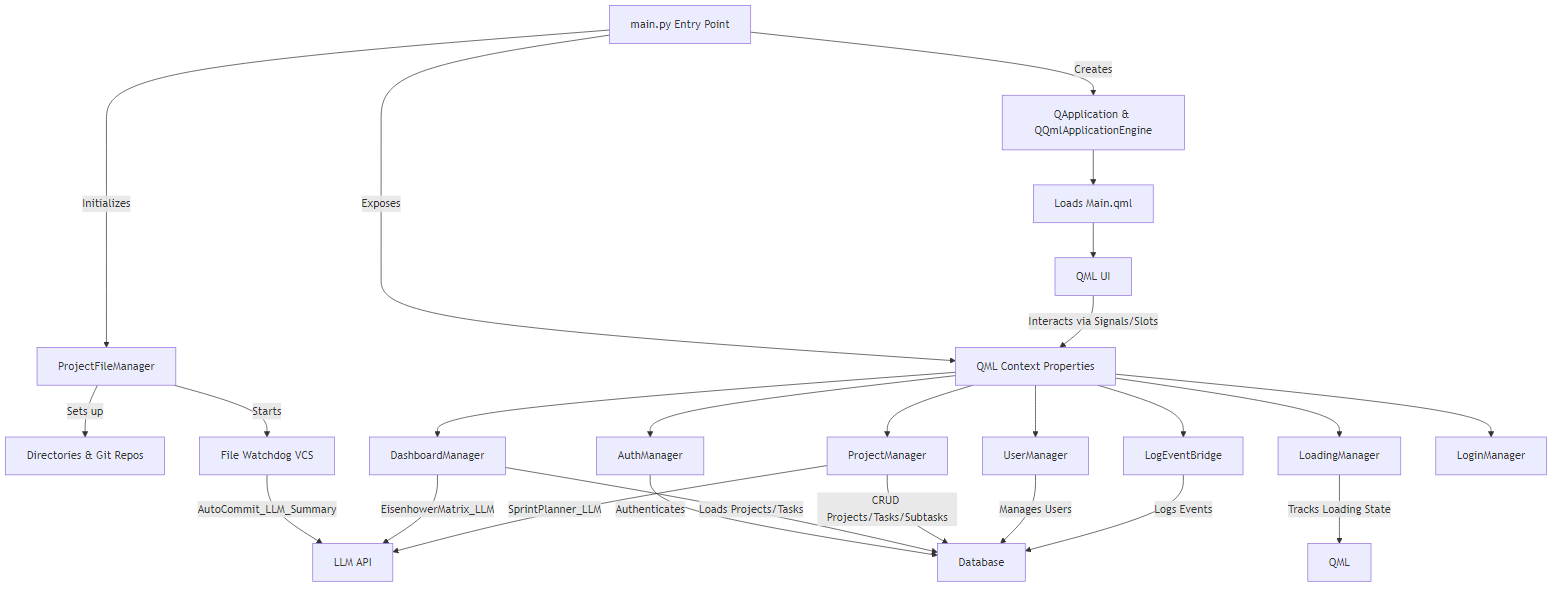
\includegraphics[width=\textwidth]{png_files/main_py_architecture.png}
\caption{Architecture diagram of \texttt{main.py} showing entry point, initialization of components, and connections to the UI.}
\end{figure}

\noindent
\textbf{Explanation:} \\
\texttt{main.py} is the application's entry point, responsible for initializing the backend (including file management and Git integration), setting up the Qt application and QML engine, and exposing Python backend objects to the QML frontend. It manages the connection between the UI and backend logic, ensuring that user actions in the interface are handled by the appropriate Python classes.

\section{Main.qml}

\begin{figure}[ht]
    \centering
    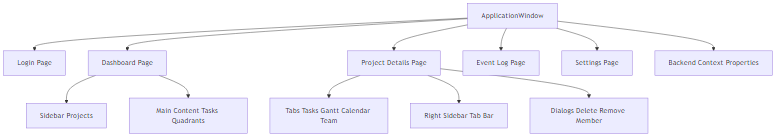
\includegraphics[width=\textwidth]{png_files/main_qml_architecture.png}
    \caption{Diagram of \texttt{Main.qml} structure, including application window, pages, navigation, and backend context properties.}
\end{figure}

\noindent
\textbf{Explanation:} \\
\texttt{Main.qml} defines the main user interface using QML. It structures the application window, navigation, and all major pages (login, dashboard, project details, event log, settings). The UI is dynamic, responding to backend signals and exposing user actions to Python logic via context properties. The dashboard and project details pages are modular, supporting tabbed navigation and dialogs for project and team management.

\section{reset\_users.py}

\begin{figure}[ht]
    \centering
    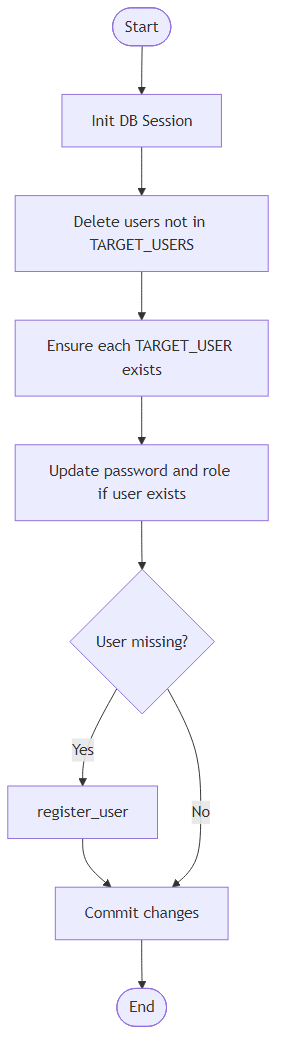
\includegraphics[width=\textwidth,height=0.8\textheight,keepaspectratio]{png_files/reset_users_flow.png}
    \caption{Diagram of \texttt{reset\_users.py} showing its interaction with the user and role tables.}
\end{figure}

\noindent
\textbf{Explanation:} \\
\texttt{reset\_users.py} is a utility script for database maintenance. It resets the user table to a predefined set of users, updating passwords and roles as needed. This ensures a consistent user base for development or testing, removing any extraneous users and enforcing correct role assignments.

\section{print\_users.py}

\begin{figure}[ht]
    \centering
    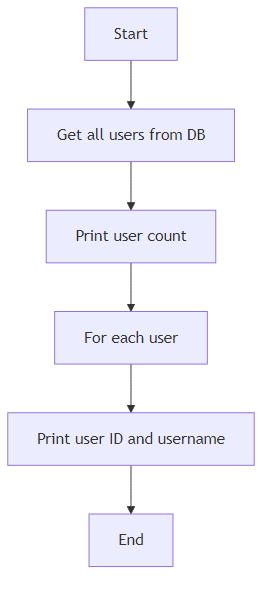
\includegraphics[width=\textwidth,height=0.8\textheight,keepaspectratio]{png_files/print_users_flow.png}
    \caption{Diagram of \texttt{print\_users.py} showing query flow for retrieving user IDs and usernames.}
\end{figure}

\noindent
\textbf{Explanation:} \\
\texttt{print\_users.py} is a simple script that queries all users from the database and prints their IDs and usernames. It is primarily used for debugging or verifying the current state of the user table.

\subsection{backend/db.py}

%\begin{figure}[ht]
%    \centering
%    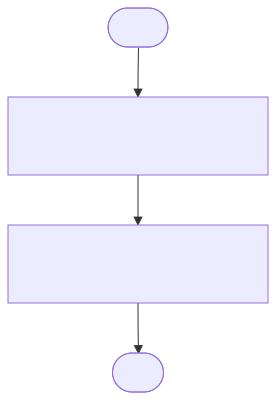
\includegraphics[width=\textwidth]{png_files/db_module_flow.png}
%    \caption{Diagram of \texttt{backend/db.py} acting as a bridge to the main application database functions.}
%\end{figure}

\noindent
\textbf{Explanation:} \\
\texttt{backend/db.py} acts as a bridge, re-exporting database functions and models from the main application database module. This allows backend logic to be organized and accessed consistently, supporting modularity and maintainability.

\chapter{User Stories}
\section{Authentication}

- As a user, I want to log in securely, so that I can access my personalized dashboard and data.
- As an admin, I want to reset the user database, so that I can ensure only authorized users have access.

\section{Project Management}
- As a user, I want to create new projects, so that I can organize my work and tasks efficiently.

- As a user, I want to view a list of all my projects, so that I can quickly access and manage them.

- As a user, I want to edit project details such as title, description, and deadline, so that project information stays up to date.

- As a user, I want to delete projects, so that I can remove obsolete or completed projects from my workspace.

\section{Team and Role Management}
- As a project owner, I want to add team members to a project and assign roles, so that I can collaborate with others.

- As a project owner, I want to remove team members, so that I can manage project access and responsibilities.

- As a project owner, I want to assign or change the project leader, so that leadership can be transferred as needed.

- As a team member, I want to view the list of project members and their roles, so that I know who is involved.

\section{Task and Subtask Management}
- As a user, I want to add tasks and subtasks to projects, so that I can break down work into manageable pieces.

- As a user, I want to assign tasks and subtasks to team members, so that responsibilities are clear.

- As a user, I want to edit and delete tasks and subtasks, so that I can keep project plans accurate.

- As a user, I want to set deadlines, durations, and dependencies for tasks and subtasks, so that project timelines are well-defined.

- As a user, I want to categorize tasks and subtasks using the Eisenhower matrix, so that I can prioritize my work effectively.
- As a user, I want to drag and drop tasks/subtasks between categories, so that I can easily update priorities.

\section{Visualisation and Planning}
- As a user, I want to view my tasks and subtasks in a dashboard, so that I can see what needs to be done today.

- As a user, I want to see a Gantt chart of project tasks and subtasks, so that I can visualize timelines and dependencies.

- As a user, I want to view a calendar with deadlines, public holidays, and personal time off, so that I can plan my work schedule.

\section{Event Logging}
- As a user, I want to see an event log of actions taken in the system, so that I can track project history and changes.

- As a user, I want to log significant actions (e.g., login, project changes, team updates), so that there is an audit trail.

\section{AI/LLM Integration}
- As a user, I want to receive AI-powered suggestions for task categorization, so that I can prioritize tasks more effectively.

- As a user, I want the system to generate commit summaries for project file changes using an LLM, so that version control messages are meaningful.

- As a user, I want to interact with local LLMs (TinyLlama, DeepSeek) for planning and suggestions, so that I can leverage AI capabilities offline.

\section{Miscellaneous}
- As a user, I want to manage my personal settings, so that I can customize my experience.

- As a user, I want to log out securely, so that my account remains protected.

\chapter{Screenshots and Interface Designs}

\end{document}